% vim:et:ts=2:
% diese Datei enthaelt den eigentlichen Vortrag, siehe Handbuch zur Latex "Beamer" Klasse

\mode<presentation> {
  \usetheme{RWTHRZ}
}

\usepackage[german]{babel}
\usepackage[utf8]{inputenc}
\usepackage{times}
\usepackage[T1]{fontenc}
\usepackage[right]{eurosym}
\usepackage{graphicx}
\usepackage{hyperref}
\definecolor{darkblue}{rgb}{0,0,.5}
\hypersetup{pdftex=true, colorlinks=true, breaklinks=true, linkcolor=darkblue, menucolor=darkblue, pagecolor=darkblue, urlcolor=darkblue}
\setbeamertemplate{navigation symbols}{}

\title[Einführung in git]{Einführung in git}
\author[Gilger, Lederhofer]{}
\date[\today]{\today}

\begin{document}

\begin{frame}
  \begin{center}
  \vspace{1cm}
  \Huge Einführung in git \\
  \vspace{1cm}
  
\includegraphics[scale=0.4]{img/git-logo.png} \\
  \vspace{0.6cm}
  \Large Johannes Gilger \& Matthias Lederhofer \\
  \small Rechen- und Kommunikationszentrum der RWTH Aachen \\
  \small Network Operation Center \\
  \vspace{1cm}
  \small 14. Juli 2010
  \end{center}
\end{frame}

\begin{frame}
  \frametitle{Übersicht}
  \begin{itemize}
    \item Begriffe in der Versionsverwaltung
    \item Unterschiede zentrale und dezentrale VCS
    \item Warum man git benutzen sollte
    \item Wie git funktioniert
    \item Wie wir git benutzen
    \item Weiterführende Literatur und Software
  \end{itemize}
\end{frame}


\begin{frame}
  \frametitle{Begriffe}
  \begin{itemize}
    \item {\bf DVCS, VCS, SCM} - (Verteilte) Versionsverwaltung
    \item {\bf Repository} - Enthält die Geschichte (alle Versionen) eines Projekts
    \item {\bf Commit, Revision} - Identifiziert eine Version \\ SVN: 423, git: {\tt b8bba41...}
    \item {\bf Branch} - Ein Entwicklungszweig in der Geschichte
    \item {\bf Worktree} - Das aktuelle Arbeitsverzeichnis (Dateien)
    \item {\bf Checkout} - Die angelegten Dateien die einem bestimmten Stand entsprechen
  \end{itemize}
\end{frame}

\begin{frame}
  \frametitle{Zentrale Versionskontrolle ...}
  \begin{center}
    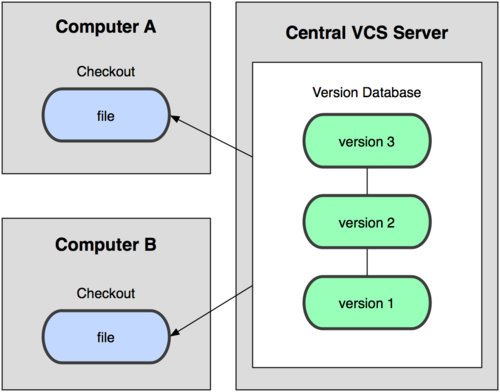
\includegraphics[width=8cm]{img/central_vcs.png}
  \end{center}
\end{frame}

\begin{frame}
  \frametitle{Dezentrale Versionskontrolle}
  \begin{center}
    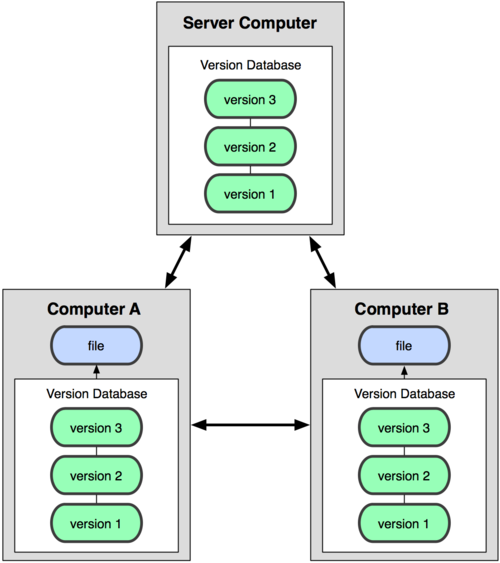
\includegraphics[width=6.3cm]{img/distributed_vcs.png}
  \end{center}
\end{frame}

\begin{frame}
  \frametitle{Typischer zentralisierter Workflow}
  \begin{center}
    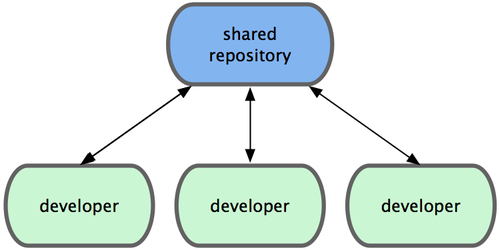
\includegraphics[width=9cm]{img/centralized_workflow.png}
  \end{center}
\end{frame}

\begin{frame}
  \frametitle{Typischer verteiler Workflow}
  \begin{center}
    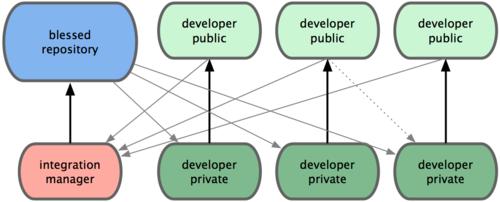
\includegraphics[width=10cm]{img/distributed_workflow.png} \\
    \vspace{0.5cm}
    Festlegung auf Master-Repository ist nur Konvention.
  \end{center}
\end{frame}

\begin{frame}
  \frametitle{Kurze Geschichte von git}
  \begin{itemize}
    \item {\bf 2005:} Linus Torvalds schreibt git für die Entwicklung des Linux-Kernels \\ Anfangs sehr low-level und kompliziert
    \item {\bf 2005-2010:} Linus gibt die Entwicklung ab, schnell wachsende und aktive Community
    \item {\bf 2010:} git 1.7.1.1 ist aktuell, viele Open-Source Projekte sind inzwischen auf git umgestiegen \\ Android, Debian, Eclipse, Fedora, GIMP, Gnome, openSUSE, Perl, Ruby on Rails, Samba, VLC, Wine, X.org
    \end{itemize}
\end{frame}

\begin{frame}
  \begin{center}
  \Huge Motivation \\
  \small {\it ''Warum die ganze Arbeit?''}
  \end{center}
\end{frame}

\begin{frame}
  \frametitle{Warum sollte man git benutzen?}
  \begin{itemize}
    \pause
    \item Viele neue Konzepte, anfangs evtl.\ schwer zu verstehen \\ Ungefähr einen Monat Einarbeitungszeit, zahlt sich jedoch schnell aus
    \pause
    \item ''SVN funktioniert doch / Viele Leute benutzen noch SVN'' \\ {\tt git-svn} hilft bei der Umstellung. Die meisten OSS-Projekte wechseln auf ein DVCS
    \pause
    \item ''Ich hab nicht vor Open-Source Software zu schreiben'' \\ git ist genauso hilfreich wenn man nur allein arbeitet
    \pause
    \item Andere Gründe?
  \end{itemize}
\end{frame}

\begin{frame}
  \frametitle{Vorteile von git gegenüber SVN}
  \begin{itemize}
    \pause
    \item {\bf Geschwindigkeit} \\ git ist \emph{sehr} schnell und speicherzeffizient, alle Operationen sind lokal (offline)
    \pause
    \item {\bf Kein Setup} \\ {\tt git init} und sofort loslegen, keine Erstellung von zentralen Projekten nötig
    \pause
    \item {\bf Einfache Rechtevergabe} \\ Normale Dateisystemberechtigungen, Zugriff lokal oder z.B.\ über SSH
    \pause
    \item {\bf Schnelle parallele Entwicklung} \\ Keine Festlegung auf Regeln oder Rollen
  \end{itemize}
  Siehe auch \url{http://www.whygitisbetterthanx.com} ;)
\end{frame}

\begin{frame}
  \frametitle{''Nachteile'' von git}
  \begin{itemize}
    \pause
    \item {\bf Kein Checkout von Subdirs} \\ Kein wirklicher Nachteil, bedeutet dass man Projekte eher in einzelne Repositories aufteilt
    \pause
    \item {\bf Keine feine Rechtevergabe für Server} \\ Oft nicht nötig durch Workflow (Maintainer, Teams)
    \pause
    \item {\bf Potentielles Chaos mit mehreren Leuten} \\ Wenn sich nicht auf einen Workflow geeignigt wird
  \end{itemize}
\end{frame}

\begin{frame}
  \begin{center}
  \Huge Technischer Hintergrund \\
  \small {\it ''Behind the curtain\ldots''}
  \end{center}
\end{frame}

\begin{frame}
  \frametitle{git Datenstrukturen und Dateilayout}
  \begin{block}{Die Datenstrukturen von git zu kennen...}
    \begin{itemize}
      \item Hilft enorm die Funktion der Befehle zu verstehen.
      \item Vermeidet falsche Arbeitsabläufe.
      \item Ist kein großer Aufwand.
    \end{itemize}
  \end{block}
\end{frame}

\begin{frame}
  \frametitle{Delta-Storage vs.\ Snapshots}
  \begin{center}
    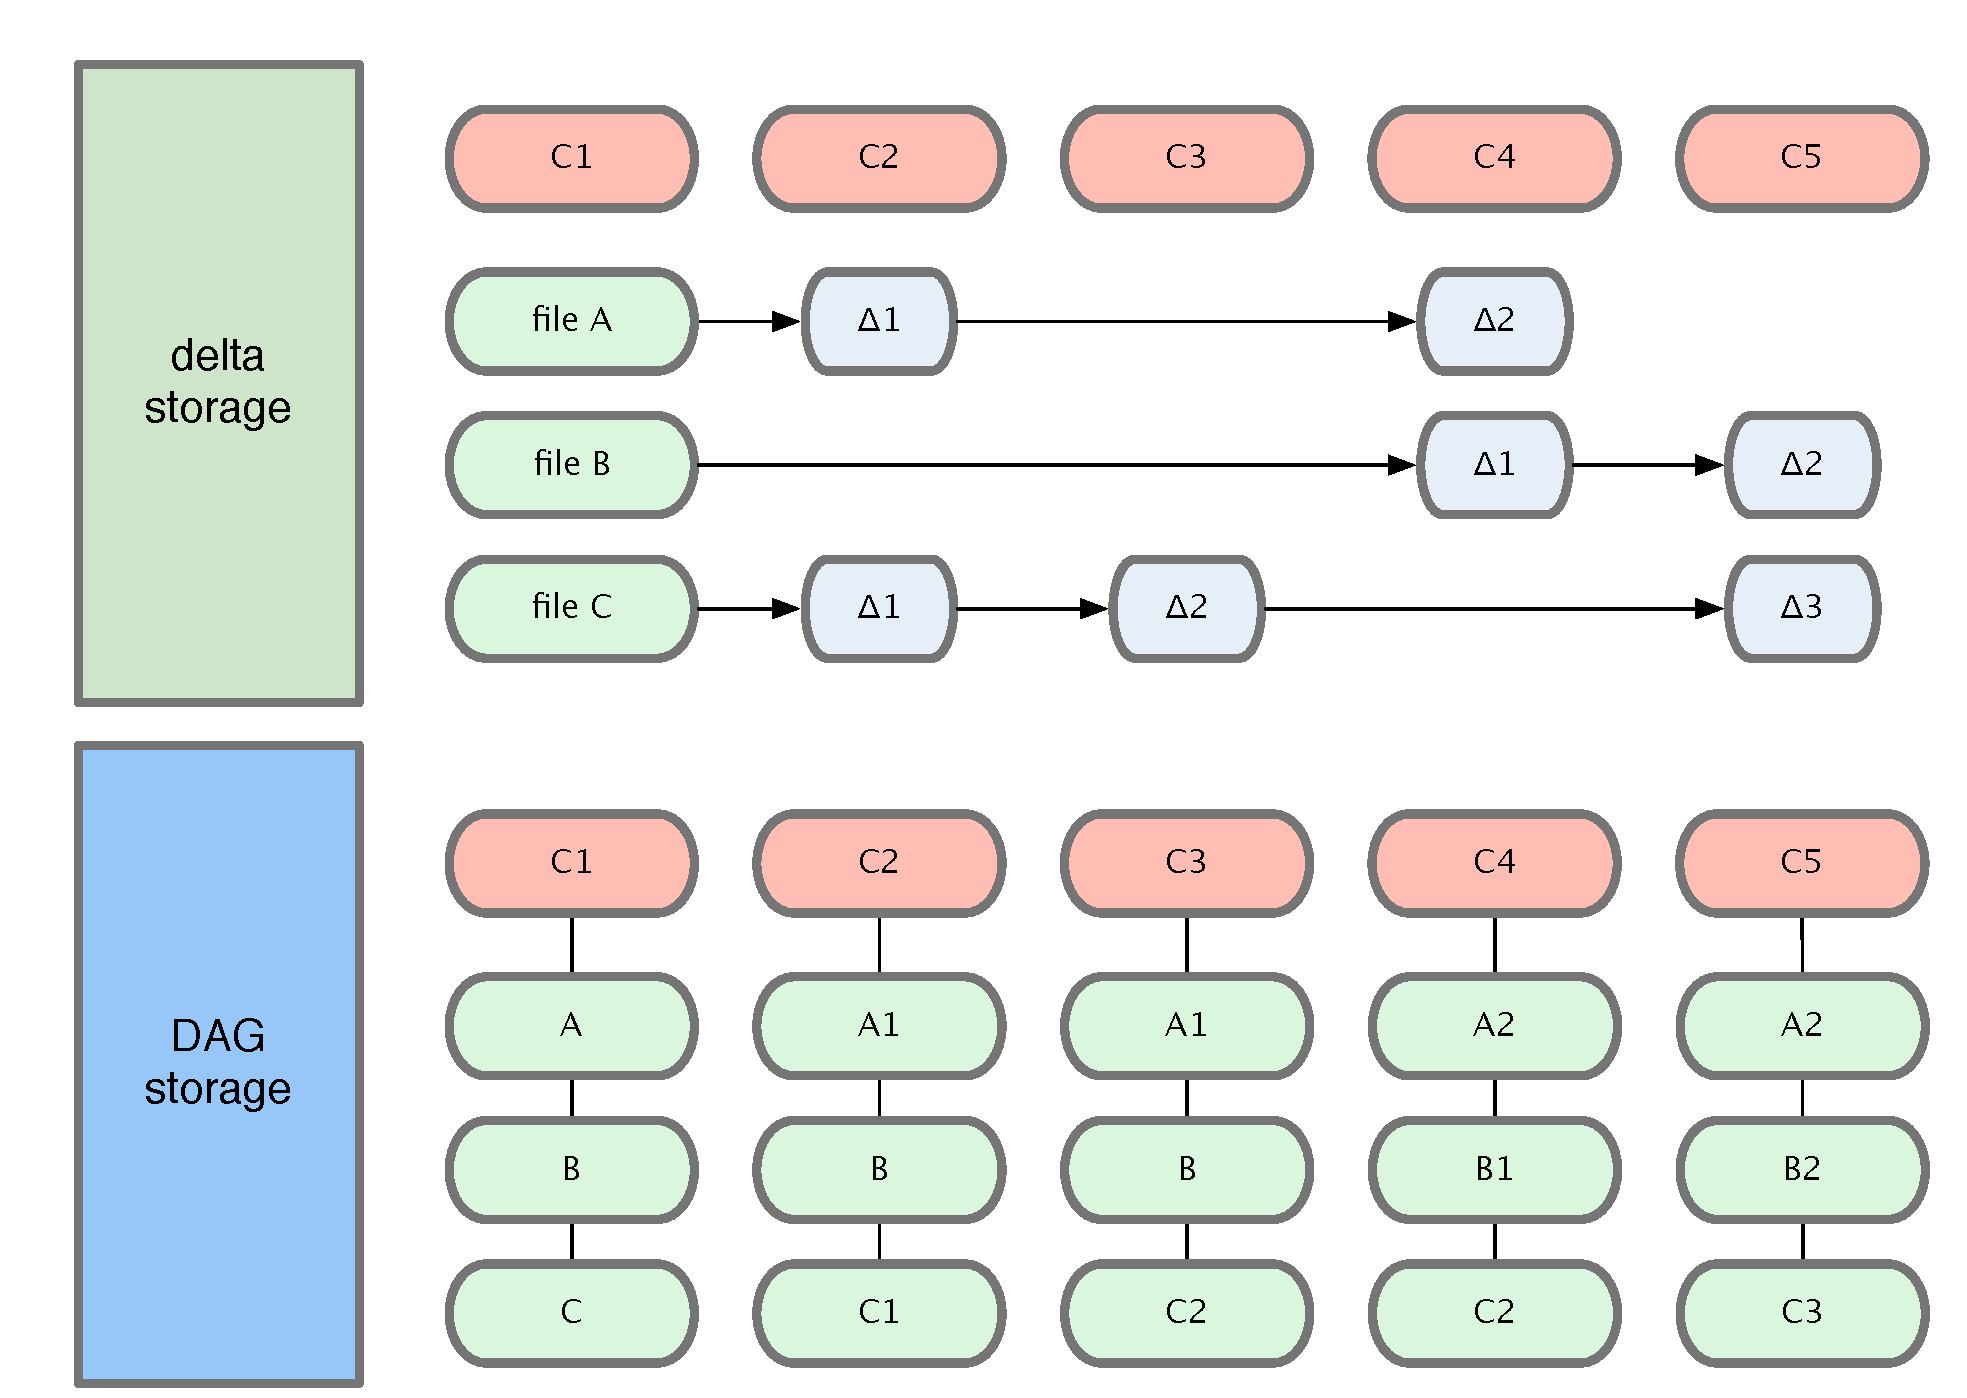
\includegraphics[width=9.5cm]{img/delta_storage.pdf}
  \end{center}
\end{frame}

\begin{frame}
  \frametitle{git ist ein Dateisystem mit Versionen}
  \begin{center}
    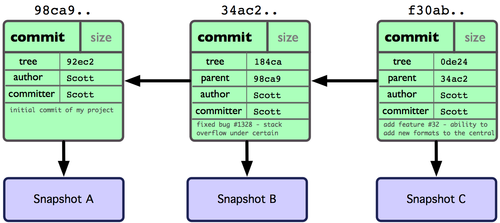
\includegraphics[width=9cm]{img/history_detailed.png} \\
    Wichtigstes Konzept: Die History ist eine einfach verlinkte Liste von Commits. Die Links zeigen ''zurück'', zeitlich gesehen.
  \end{center}
\end{frame}

\begin{frame}
  \frametitle{git ist eine Objekt-Datenbank}
  \begin{center}
    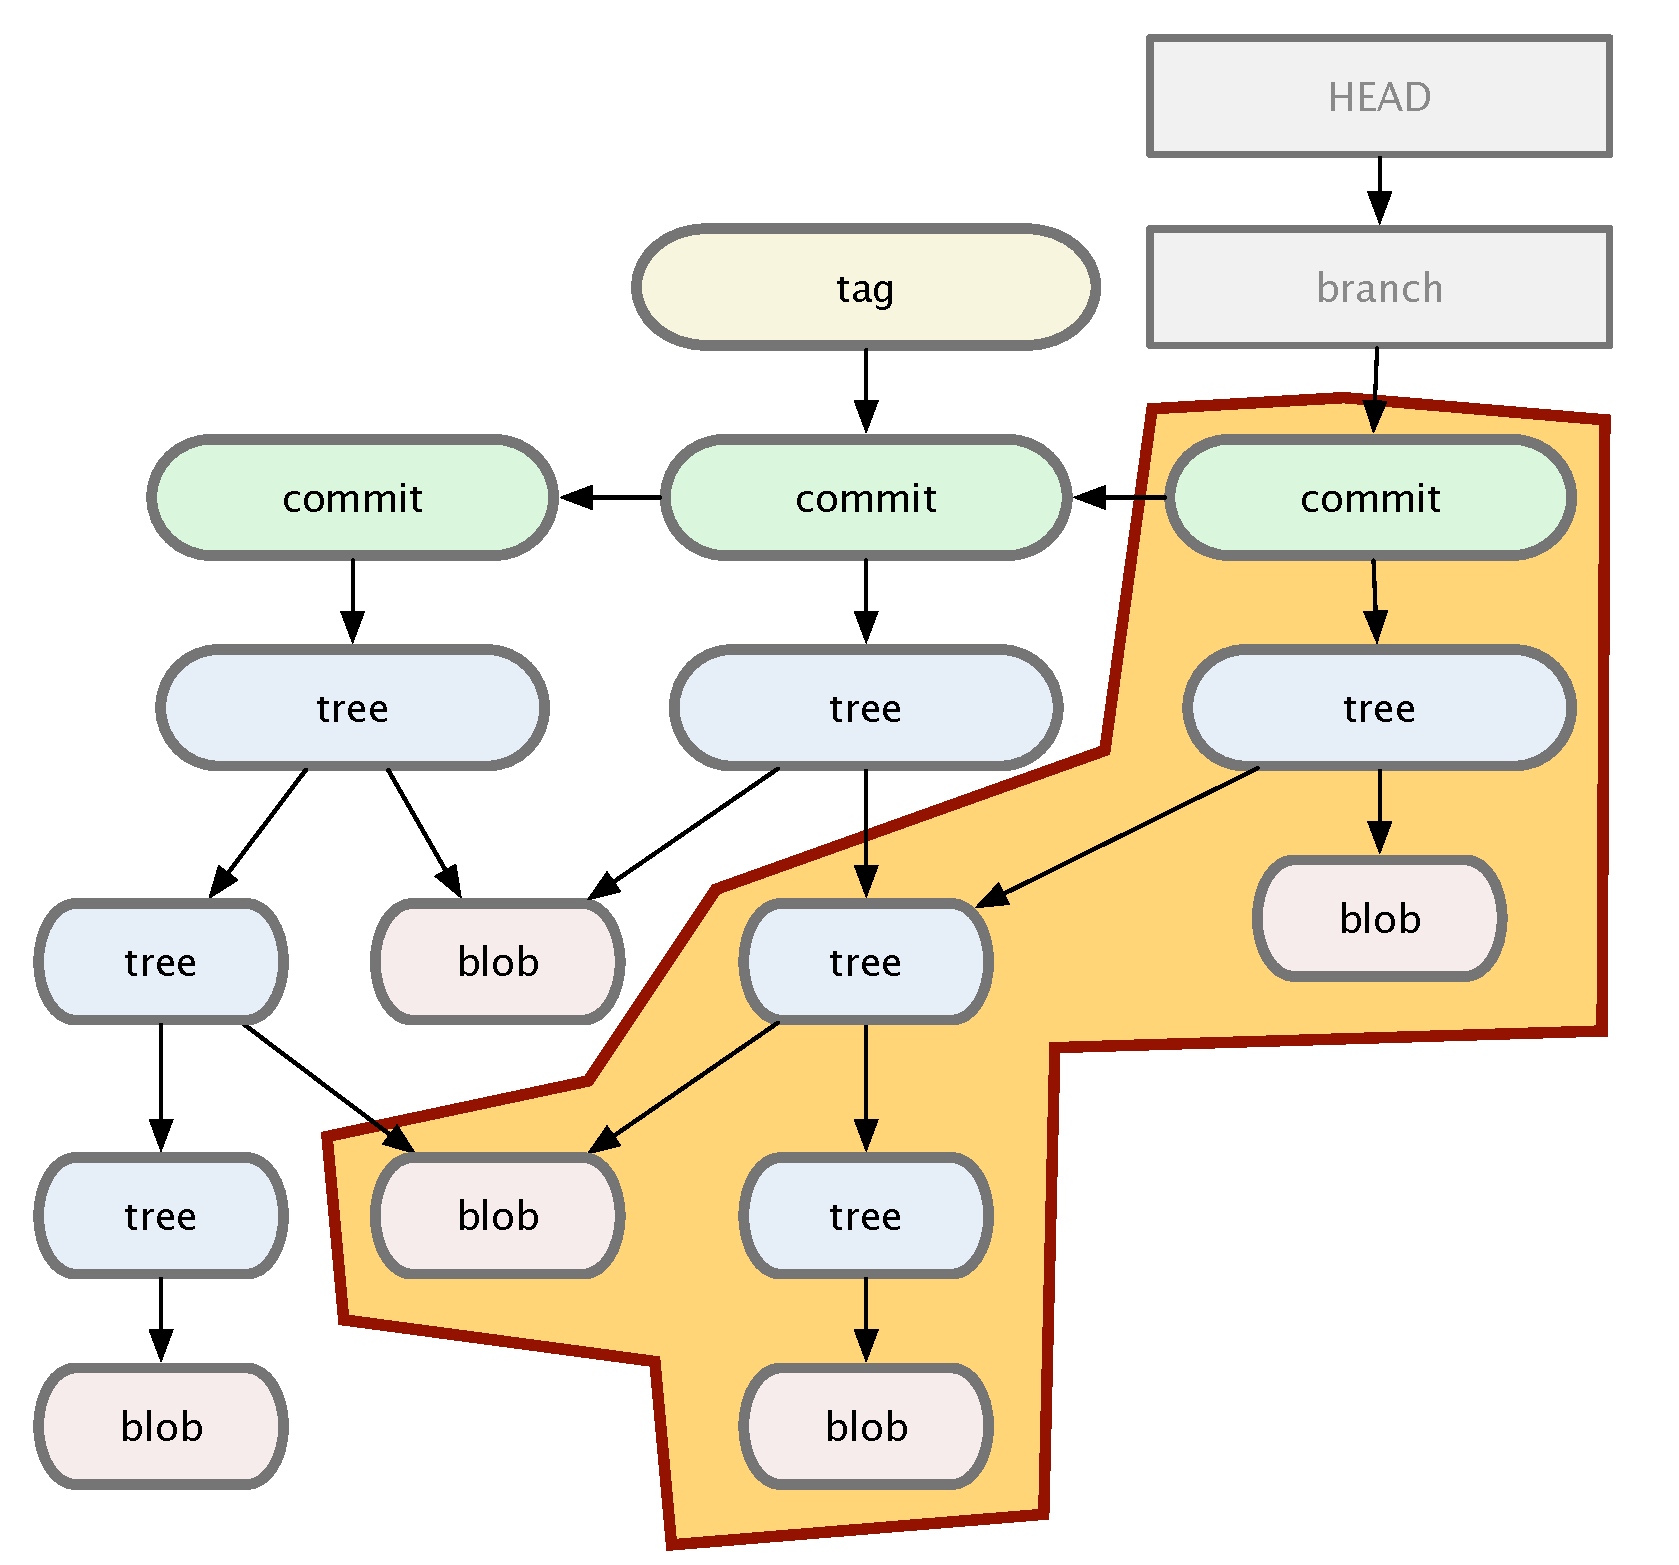
\includegraphics[width=7.8cm]{img/tree_commit.pdf}
  \end{center}
\end{frame}

\begin{frame}
  \frametitle{Commits und Branches}
  \begin{center}
    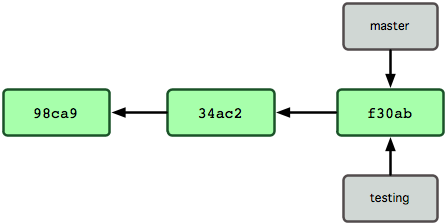
\includegraphics[width=10cm]{img/two_branches.png} \\
    Branches sind nur Zeiger (''references'') auf existierende Commits
  \end{center}
\end{frame}

\begin{frame}
  \frametitle{HEAD - der aktuelle Branch}
  \begin{center}
    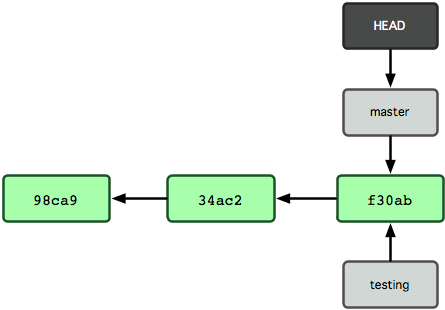
\includegraphics[width=8.5cm]{img/headref.png} \\
    HEAD zeigt an auf welchem Branch aktuell Commits gespeichert werden
  \end{center}
\end{frame}

\begin{frame}
  \frametitle{git checkout - den aktuellen Branch ändern}
  \begin{center}
    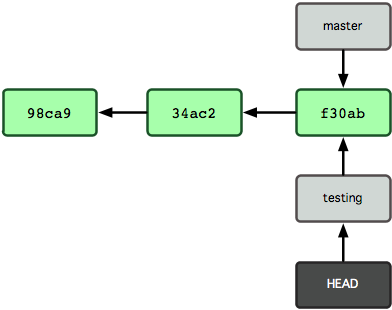
\includegraphics[width=8cm]{img/headref_changed.png} \\
    Ein Checkout aktualisiert den Worktree und den HEAD-Zeiger
  \end{center}
\end{frame}

\begin{frame}
  \frametitle{git commit - einen Commit erstellen}
  \begin{center}
    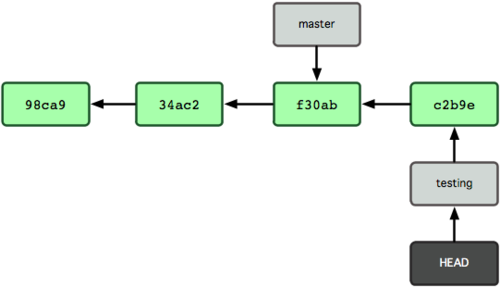
\includegraphics[width=10cm]{img/new_commit.png} \\
    Da HEAD auf ''testing'' zeigte wurde hier der Commit angelegt
  \end{center}
\end{frame}

\begin{frame}
  \frametitle{git checkout - zum ersten Branch zurück}
  \begin{center}
    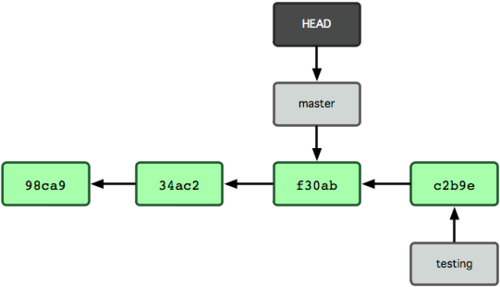
\includegraphics[width=10cm]{img/checkout.png} \\
    Es müssen währenddessen noch Änderungen am Hauptentwicklungszweig vorgenommen werden
  \end{center}
\end{frame}

\begin{frame}
  \frametitle{git commit - ein paralleler Branch}
  \begin{center}
    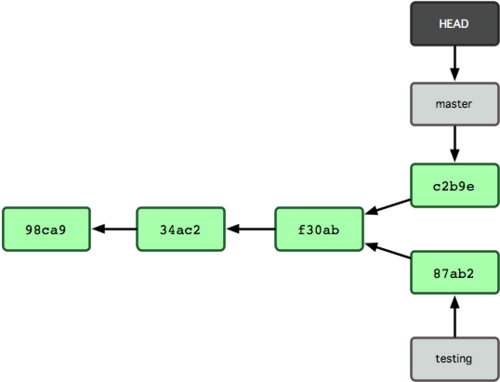
\includegraphics[width=9cm]{img/branch.png}
  \end{center}
\end{frame}

\begin{frame}
  \frametitle{Branching und Merging}
  \begin{center}
    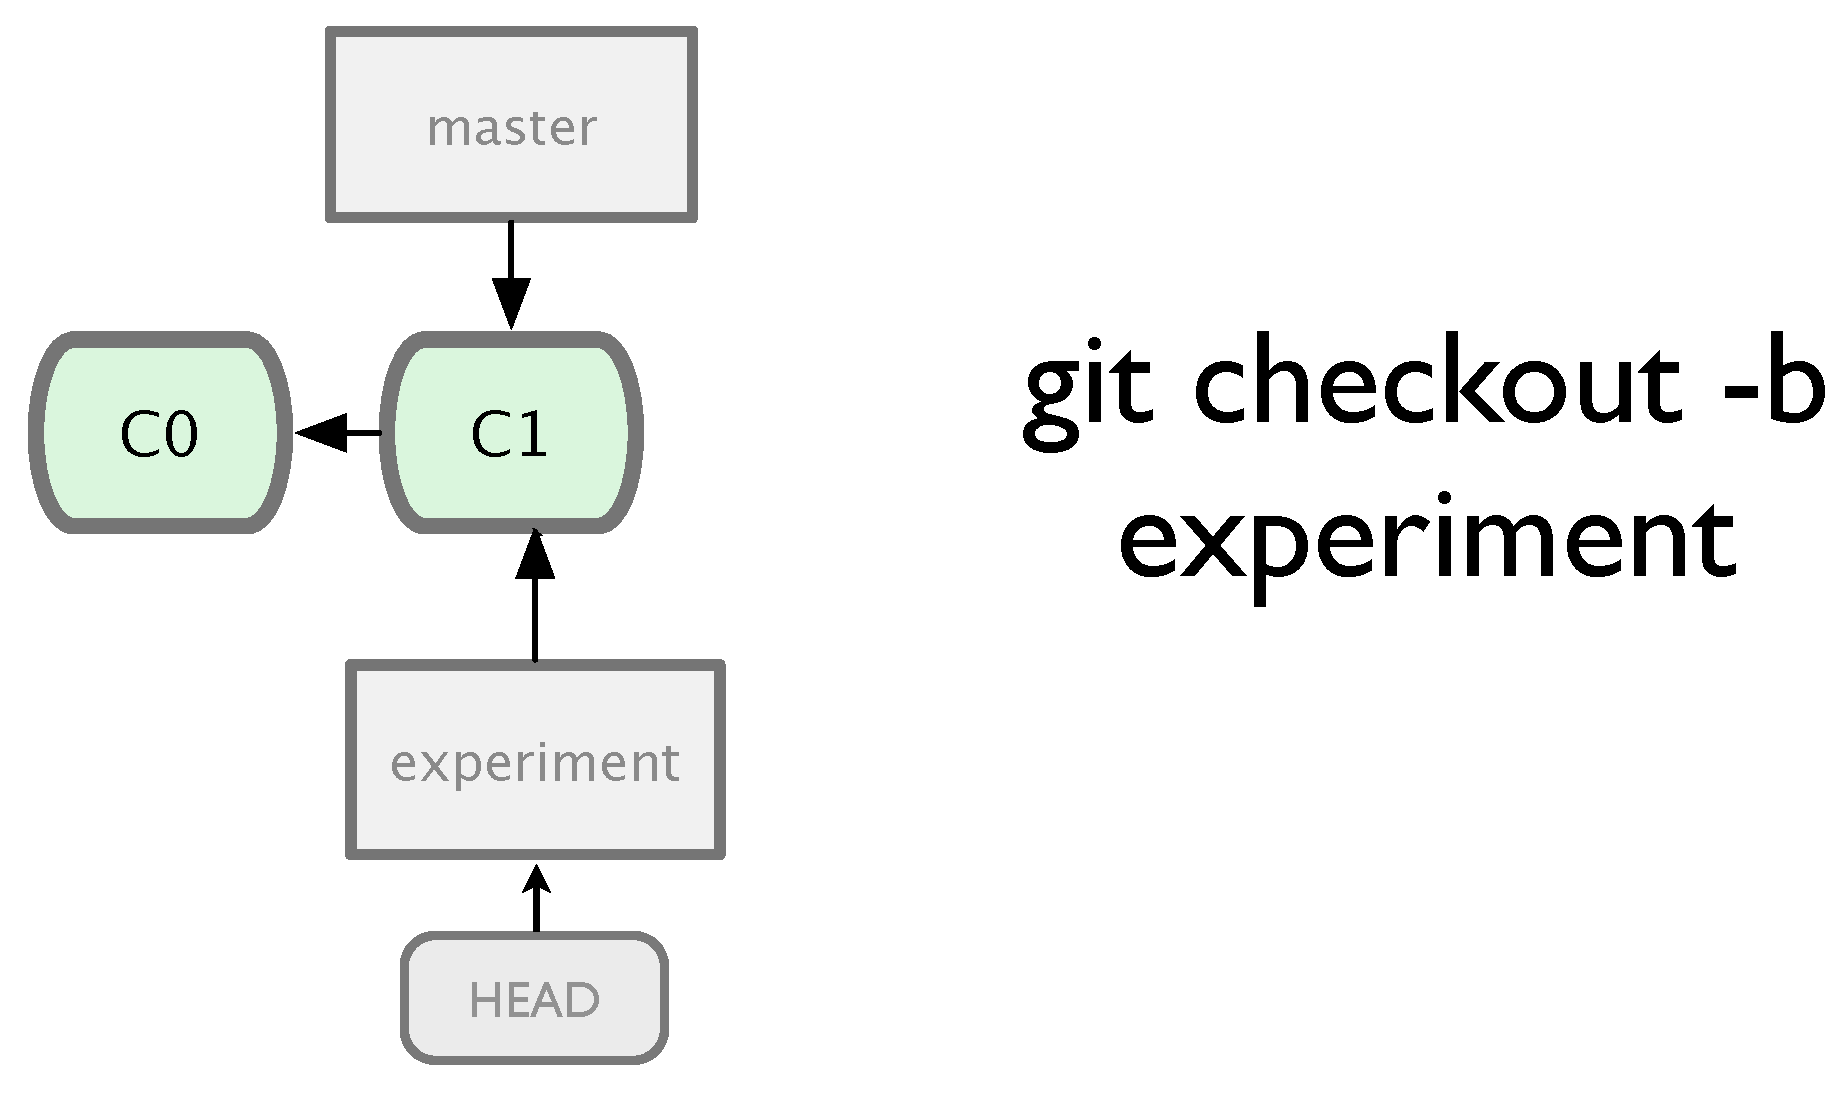
\includegraphics[width=9cm]{img/branch_1.pdf}
  \end{center}
\end{frame}

\begin{frame}
  \frametitle{Branching und Merging}
  \begin{center}
    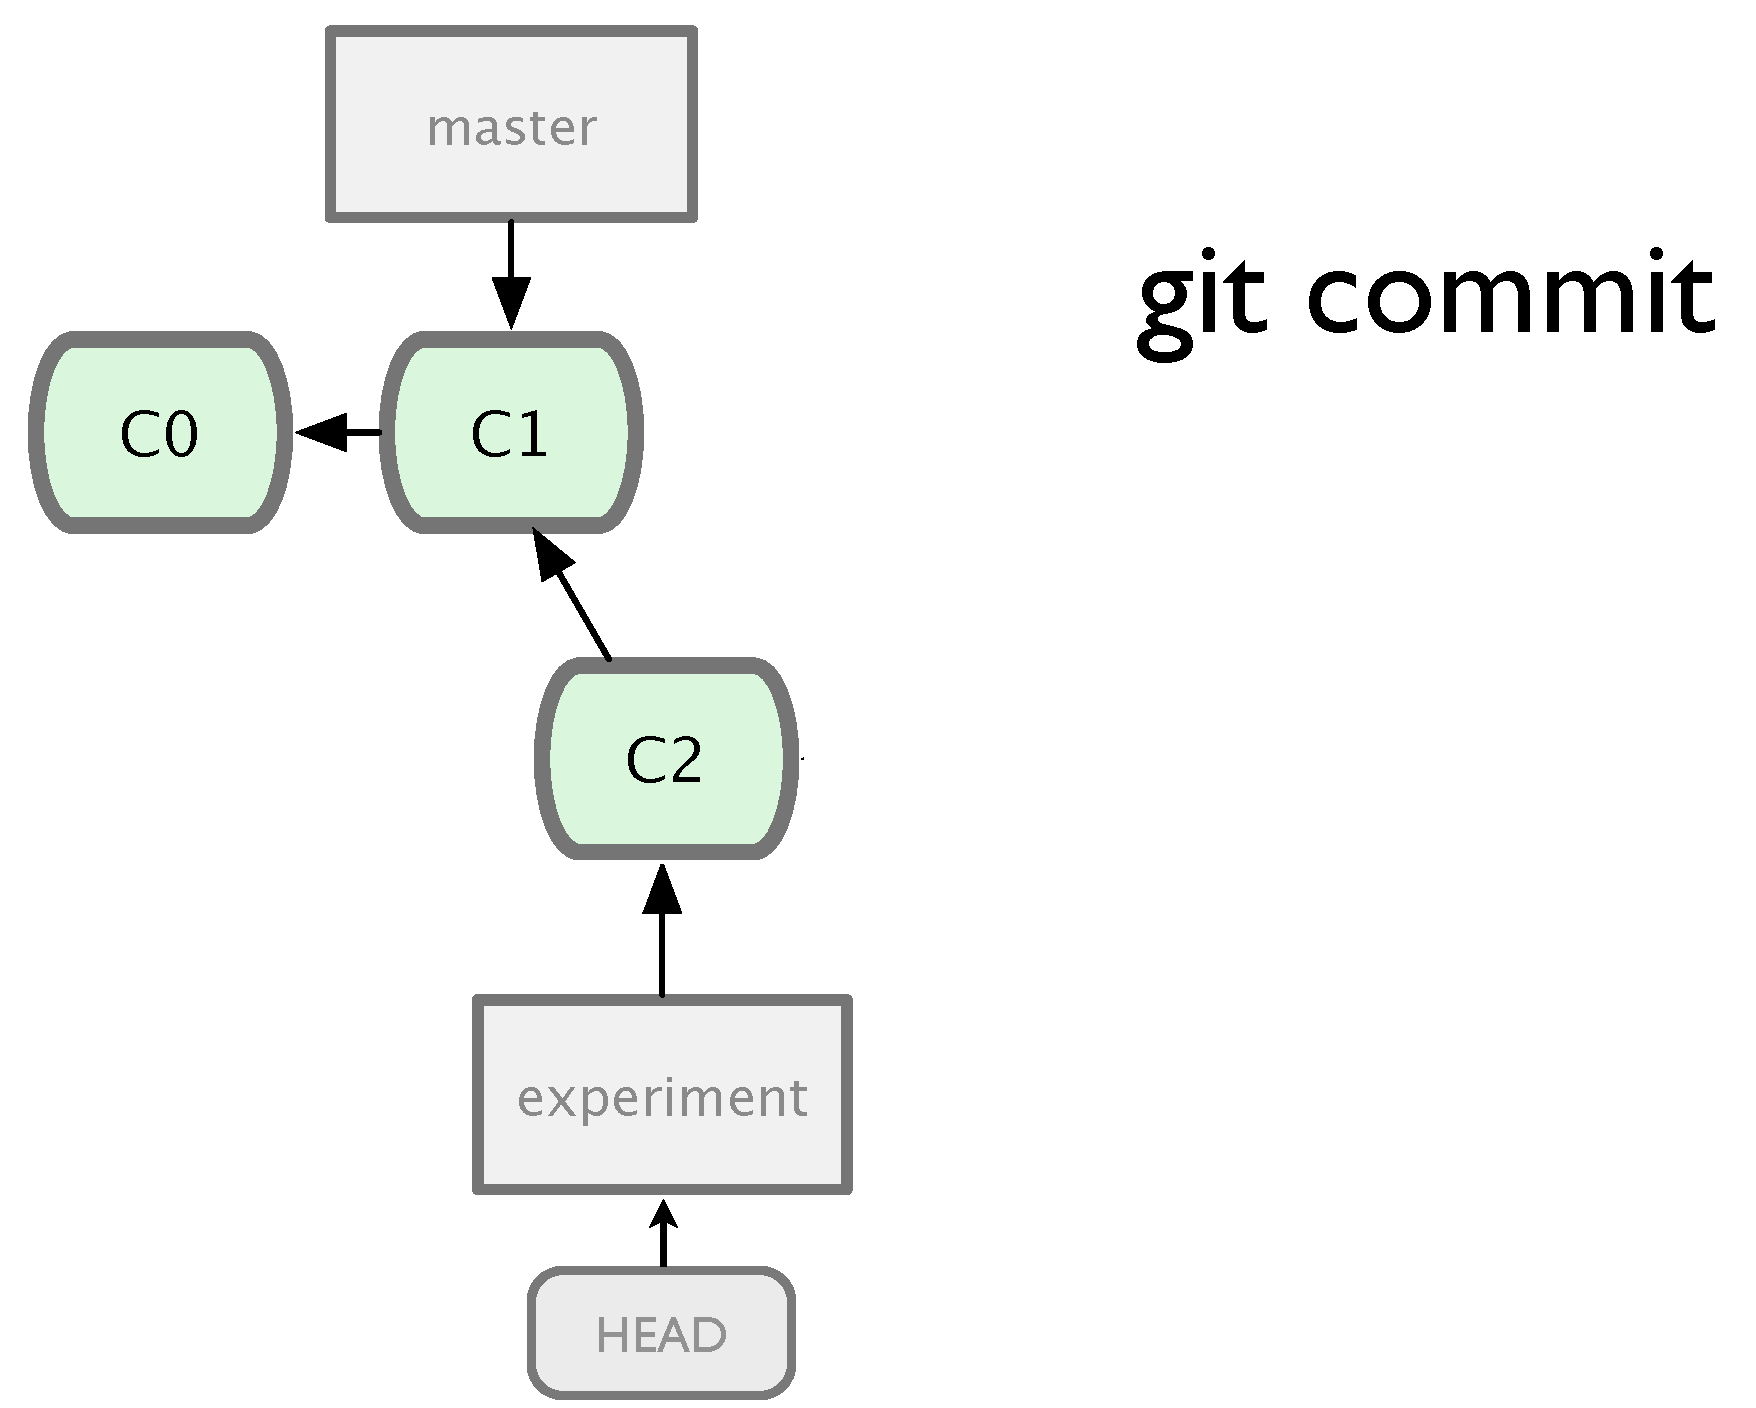
\includegraphics[width=9cm]{img/branch_2.pdf}
  \end{center}
\end{frame}

\begin{frame}
  \frametitle{Branching und Merging}
  \begin{center}
    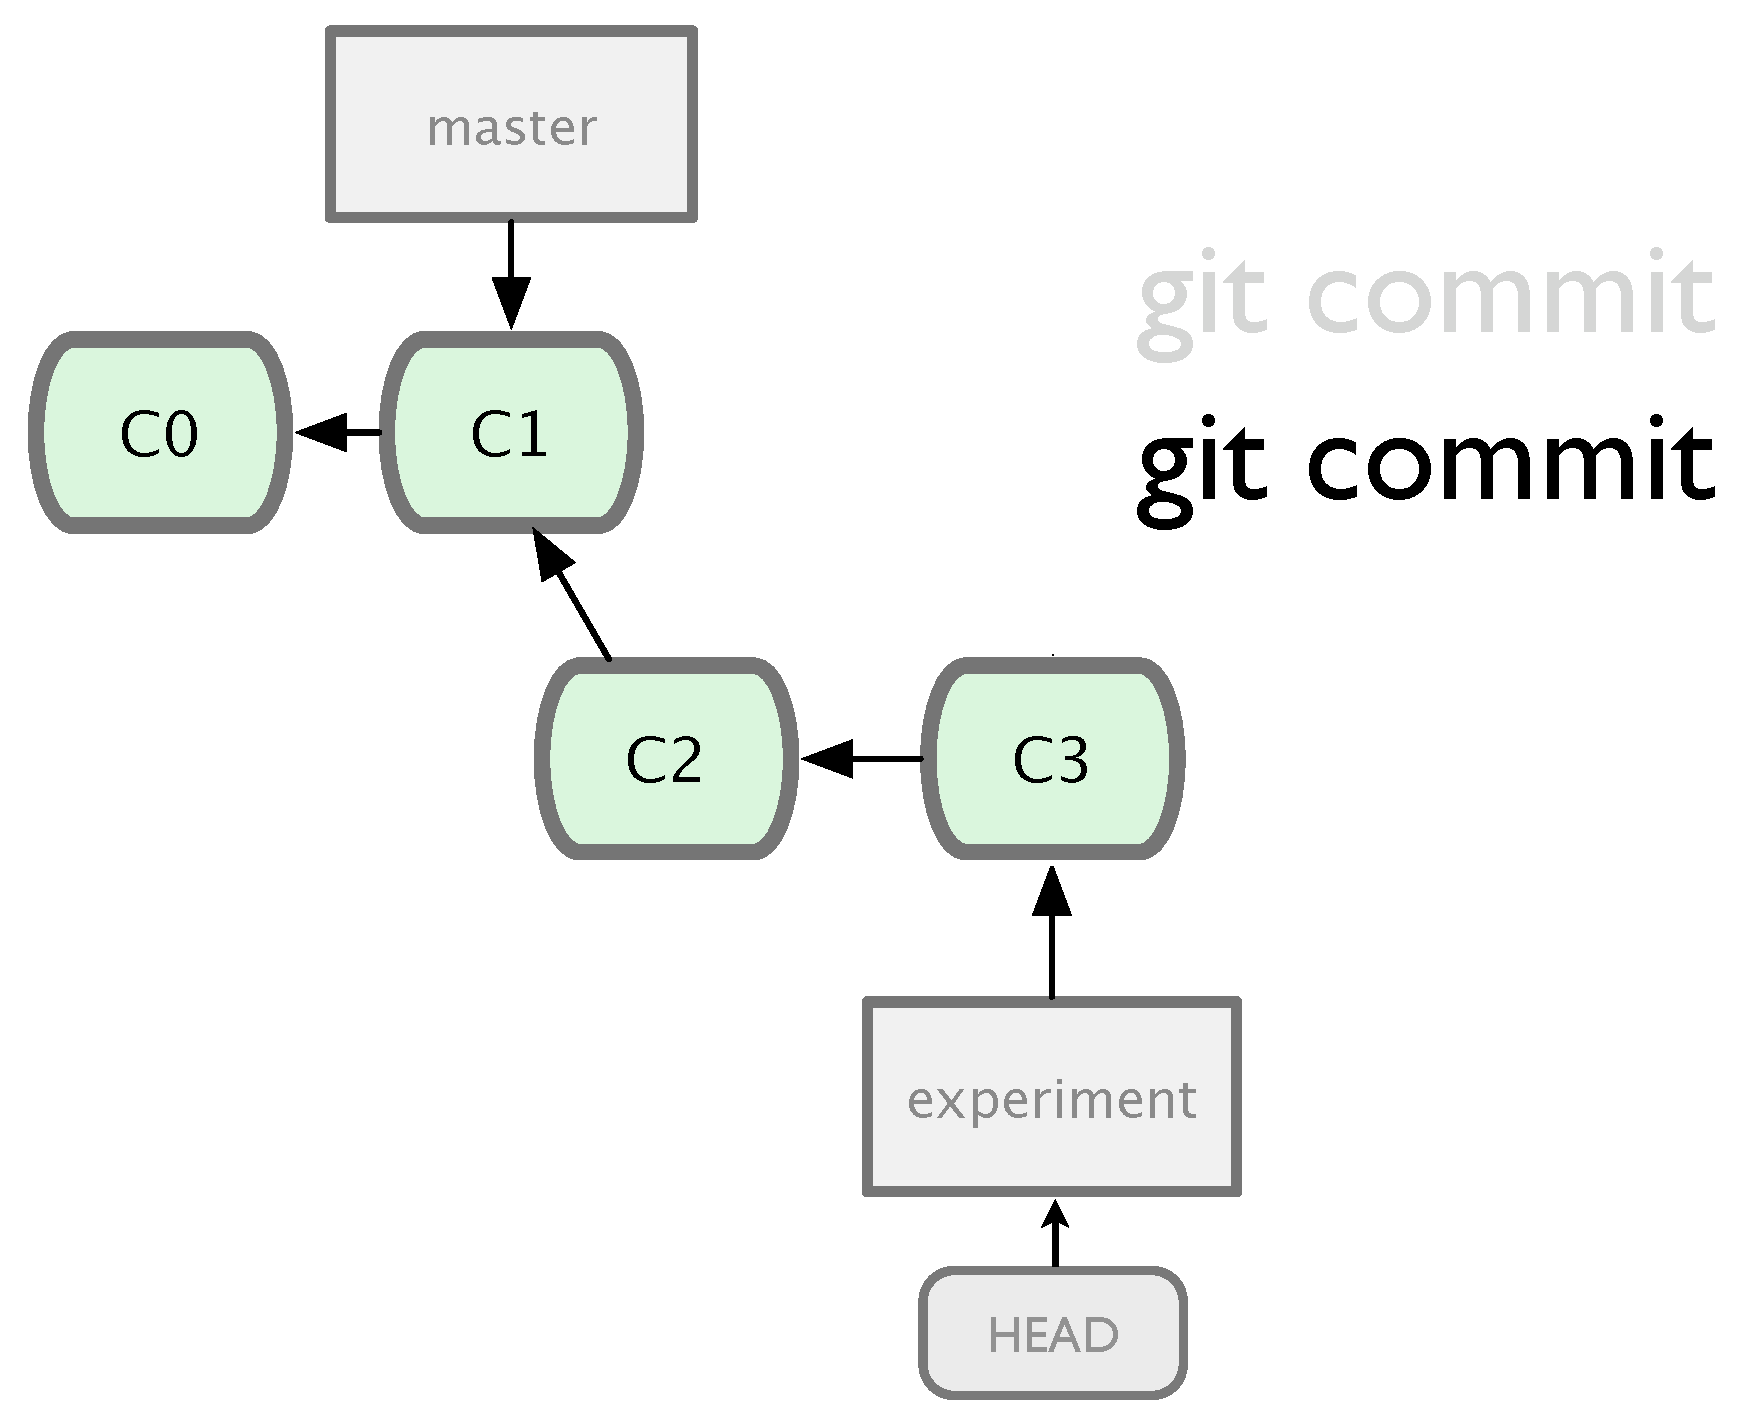
\includegraphics[width=9cm]{img/branch_3.pdf}
  \end{center}
\end{frame}

\begin{frame}
  \frametitle{Branching und Merging}
  \begin{center}
    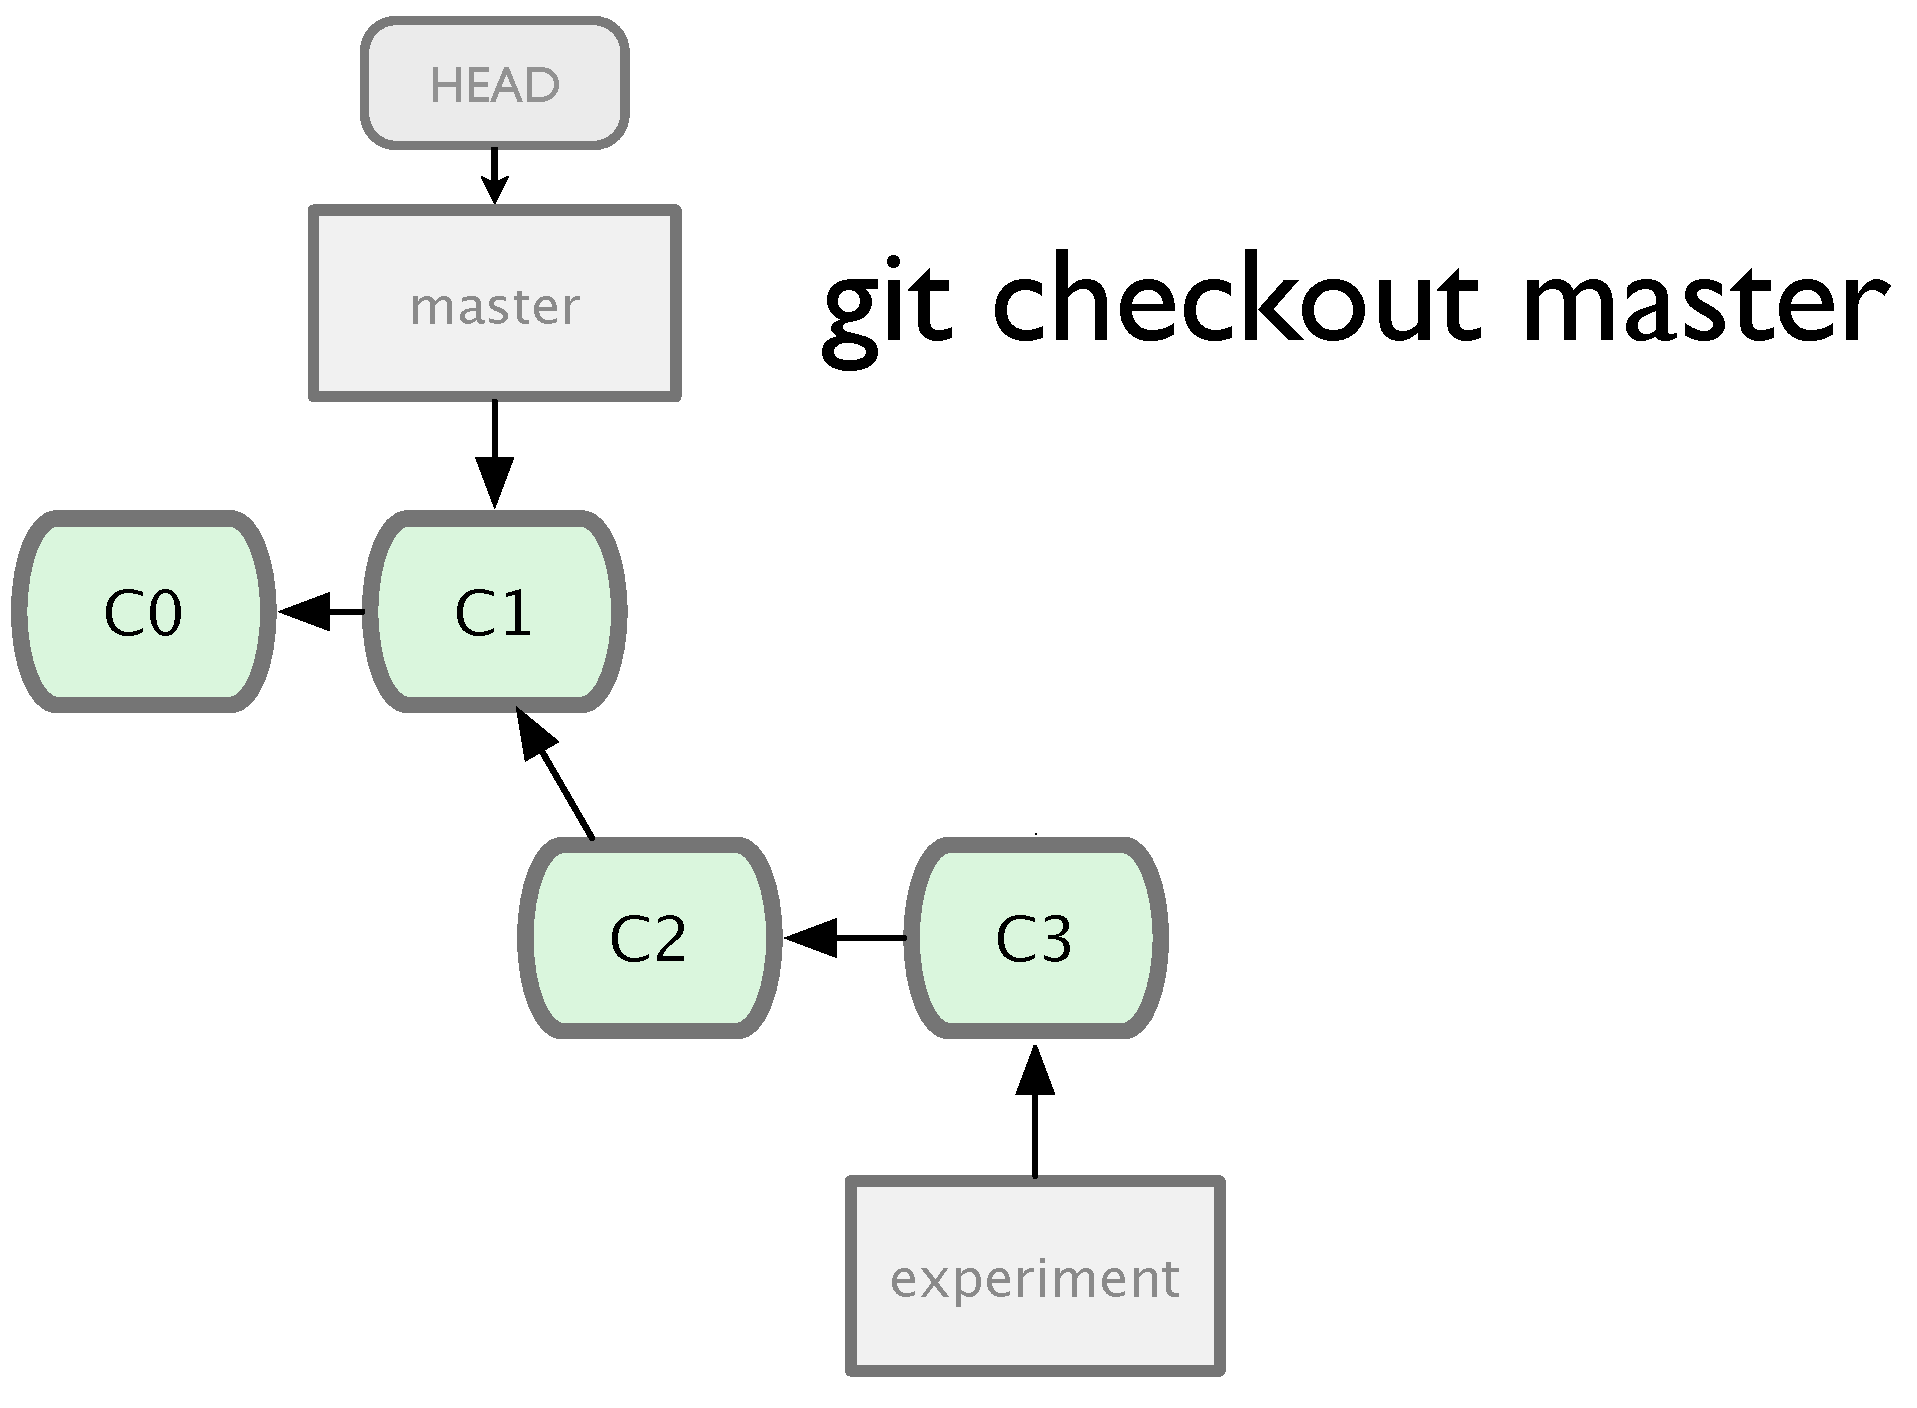
\includegraphics[width=9cm]{img/branch_4.pdf}
  \end{center}
\end{frame}

\begin{frame}
  \frametitle{Branching und Merging}
  \begin{center}
    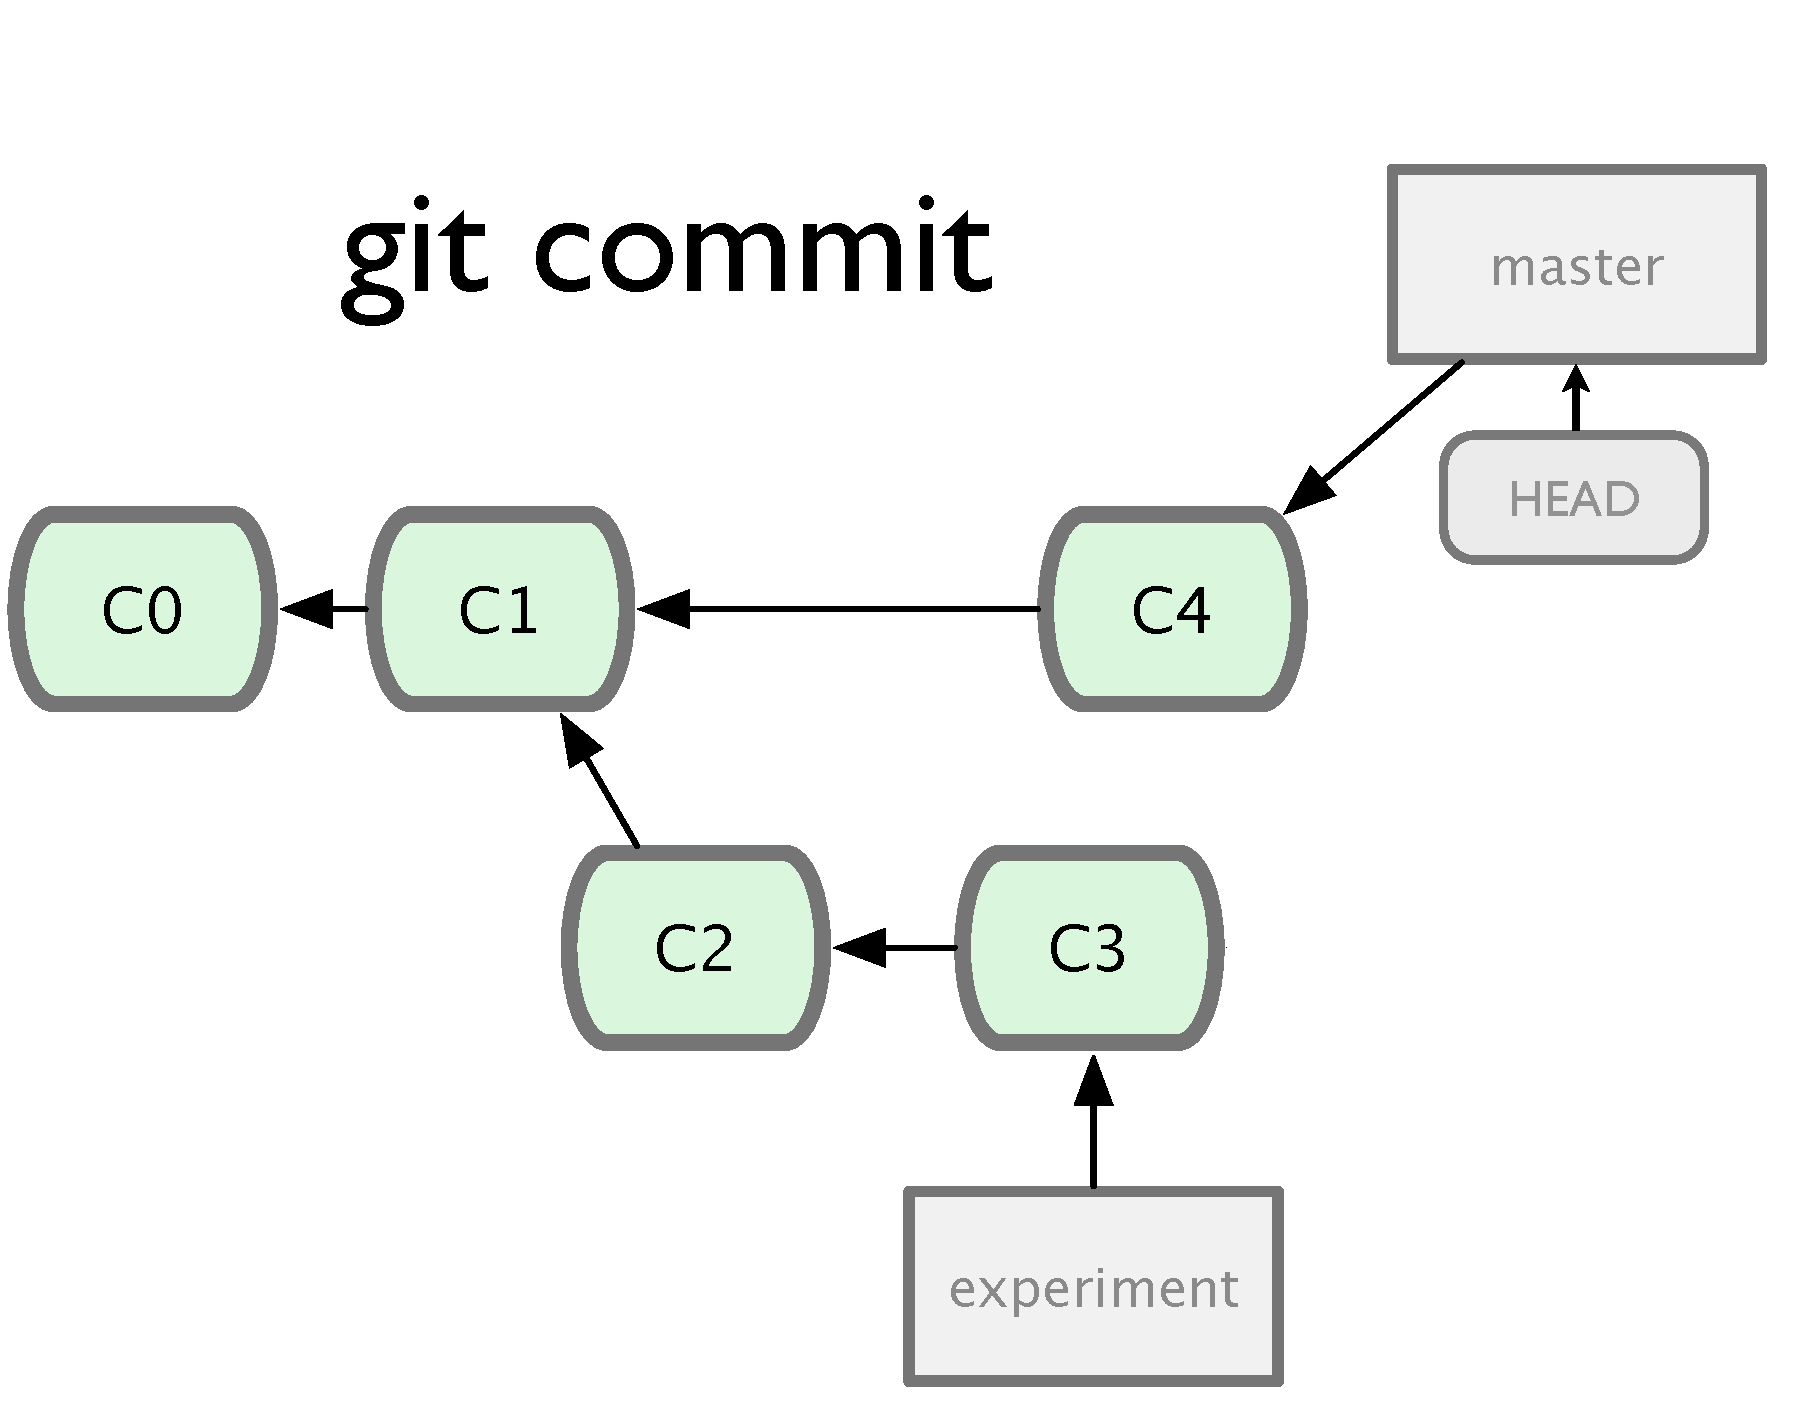
\includegraphics[width=9cm]{img/branch_5.pdf}
  \end{center}
\end{frame}

\begin{frame}
  \frametitle{Branching und Merging}
  \begin{center}
    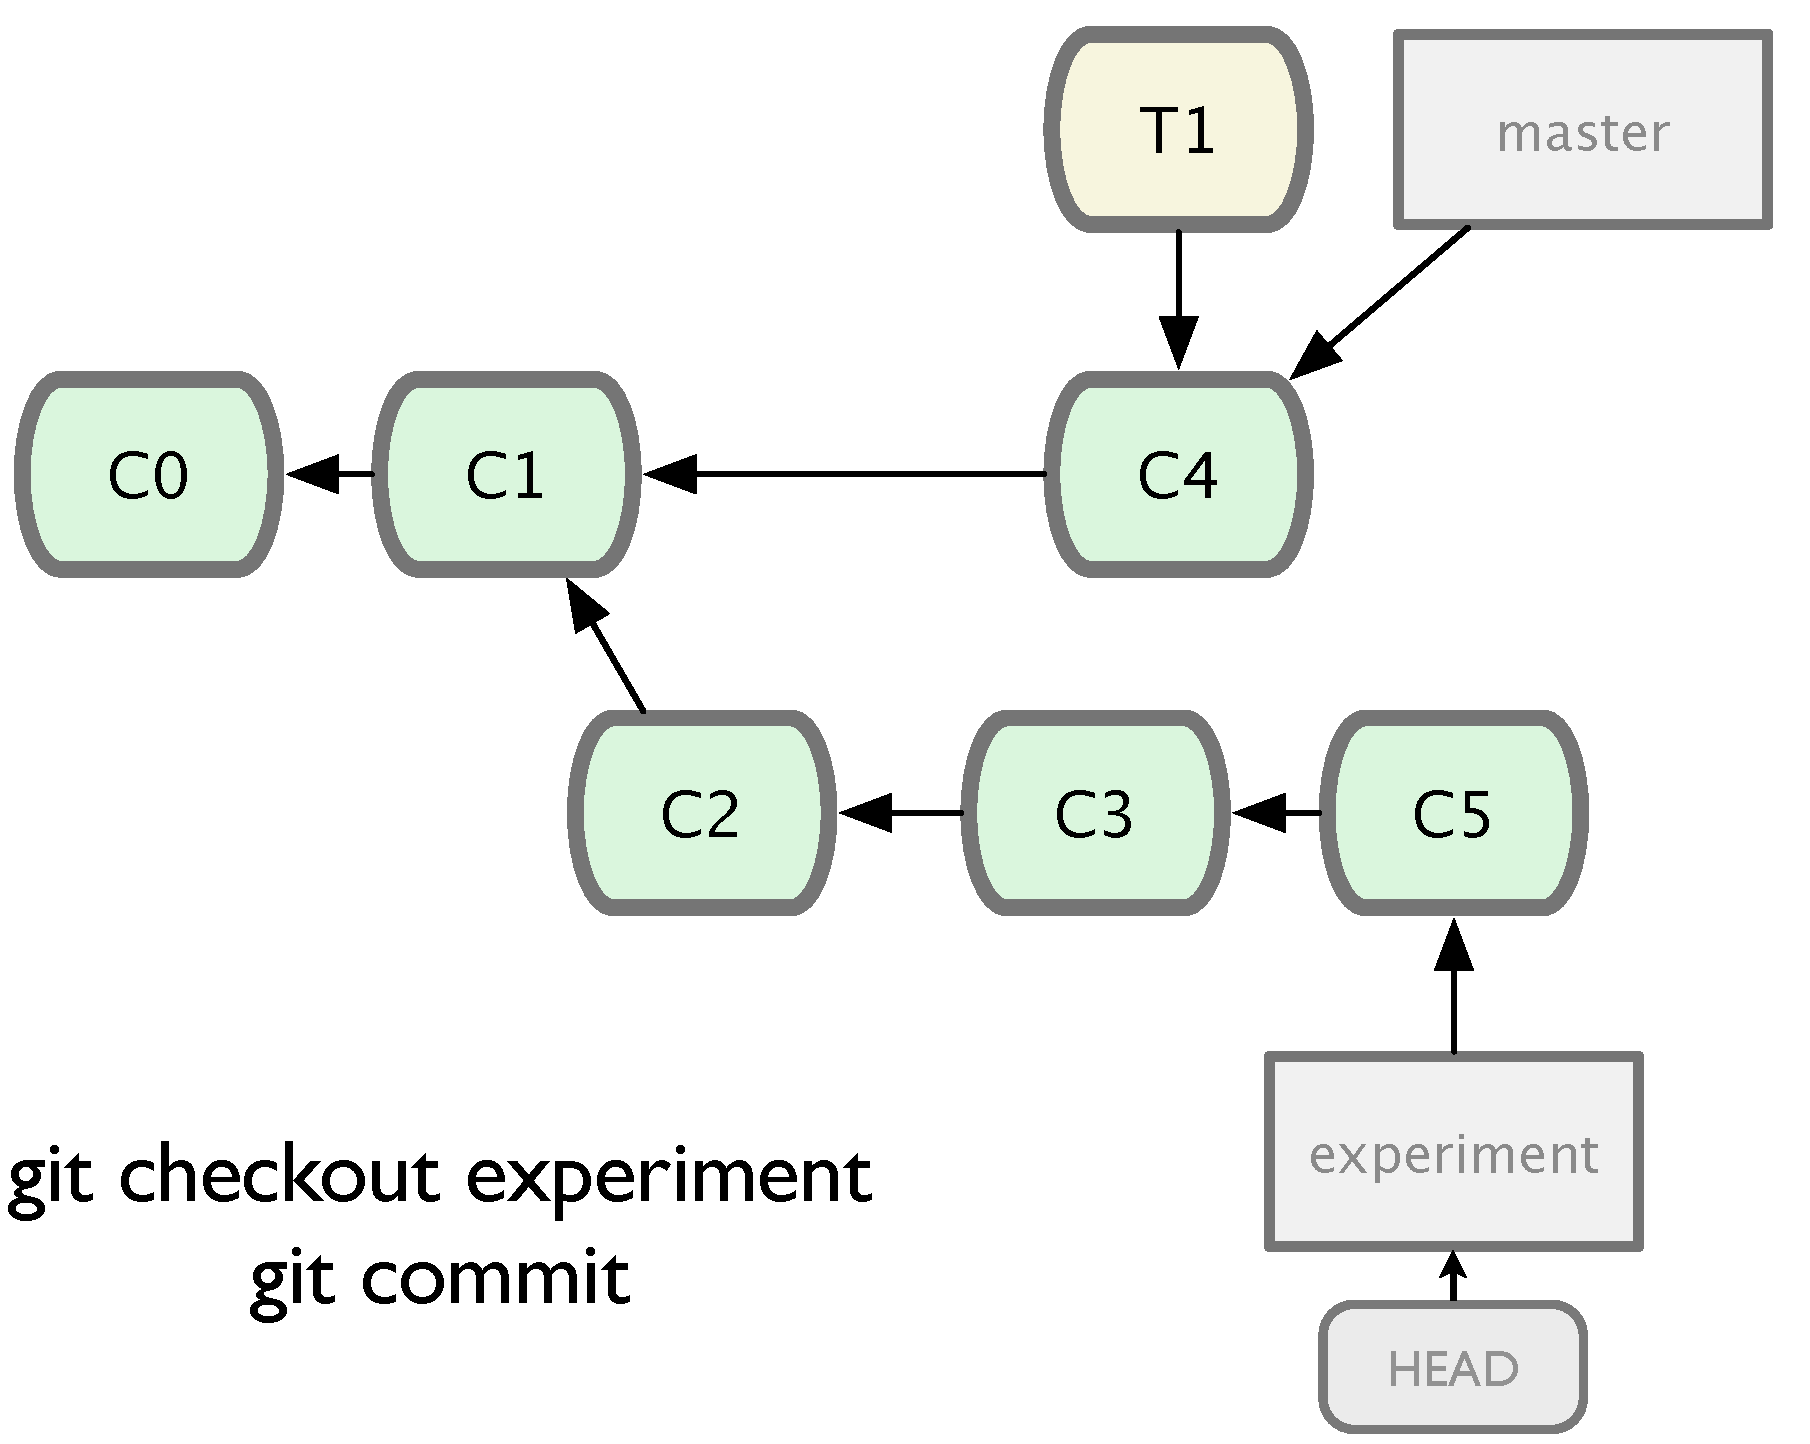
\includegraphics[width=9cm]{img/branch_6.pdf}
  \end{center}
\end{frame}

\begin{frame}
  \frametitle{Branching und Merging}
  \begin{center}
    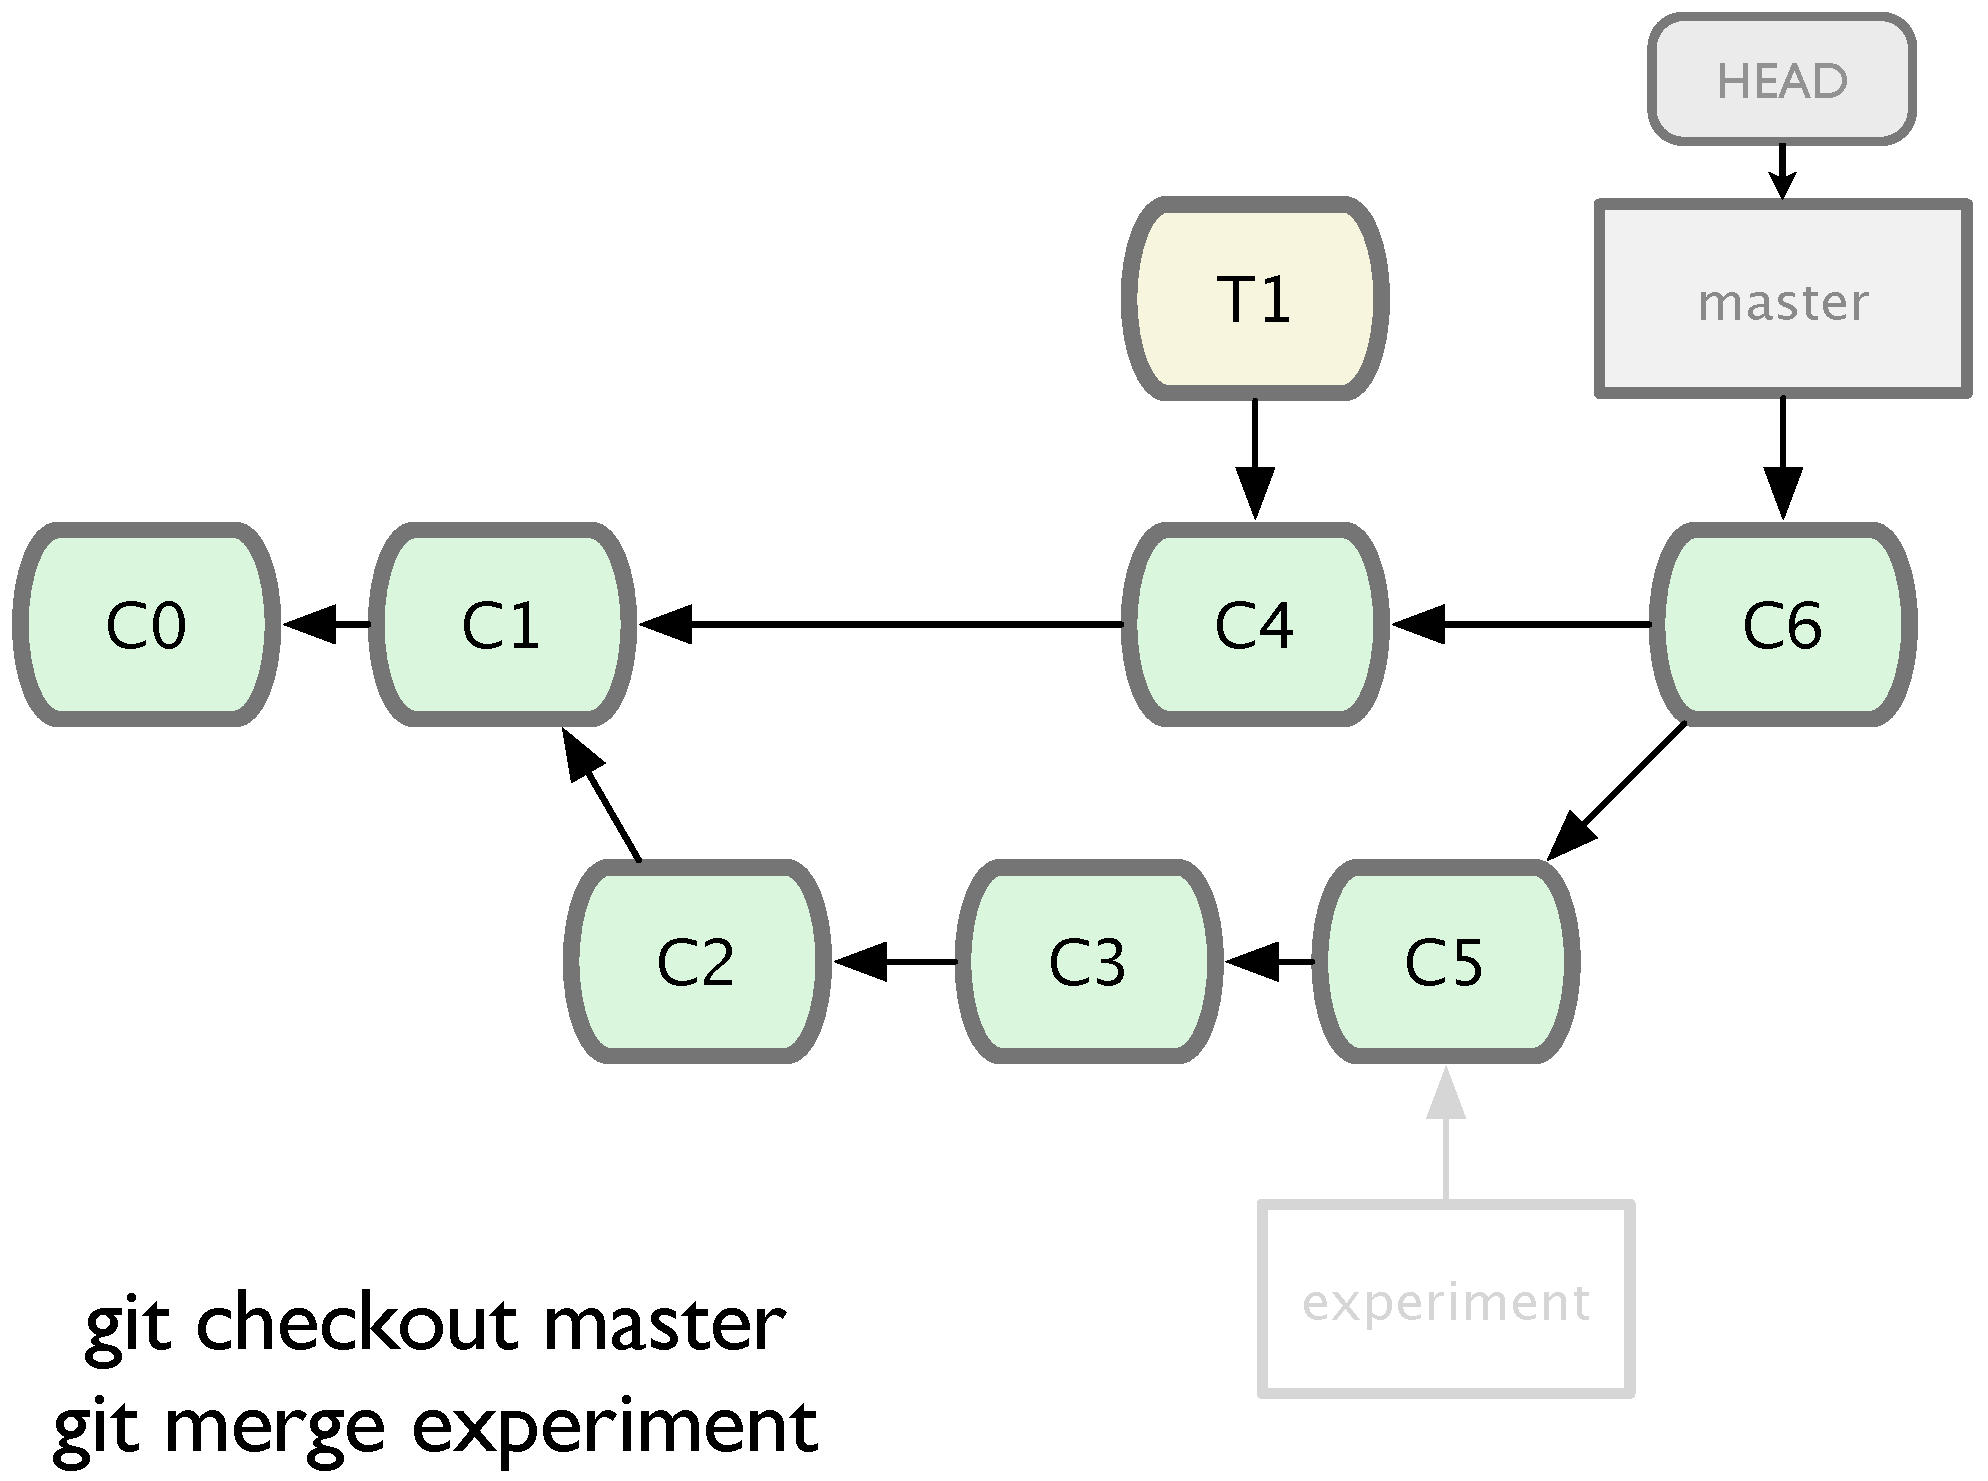
\includegraphics[width=9cm]{img/branch_7.pdf}
  \end{center}
\end{frame}

\begin{frame}
  \frametitle{Remotes}
  \begin{itemize}
    \item Remotes sind Kürzel um mit anderen Repositories zu arbeiten. Namespaces nach Repository: {\tt jojo/master}
    \item Remote Branches (Tracking Branches) dienen dazu der Arbeit in anderen Repositories zu folgen
    \item Entwickelt wird \emph{immer} auf lokalen Branches
    \item Auf Remote Branches kann nicht committed werden
    \item Remote Branches werden nur durch fetch / pull geändert
  \end{itemize}
\end{frame}

\begin{frame}
  \frametitle{Tracking Branch}
  \begin{center}
    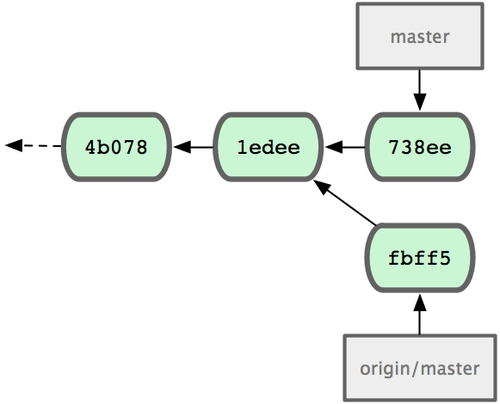
\includegraphics[width=9cm]{img/remote_1.png}
  \end{center}
\end{frame}

\begin{frame}
  \frametitle{Tracking Branch}
  \begin{center}
    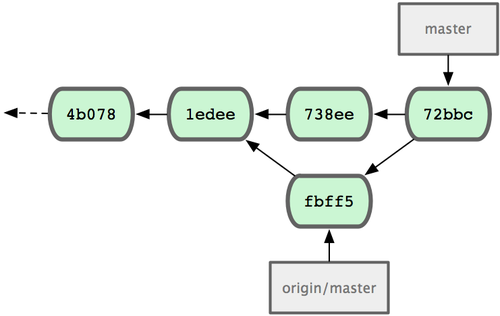
\includegraphics[width=9cm]{img/remote_2.png}
  \end{center}
\end{frame}

\begin{frame}
  \frametitle{Tracking Branch}
  \begin{center}
    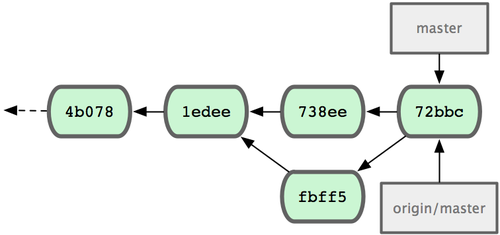
\includegraphics[width=9cm]{img/remote_3.png}
  \end{center}
\end{frame}

\begin{frame}
  \frametitle{Der Index / Stage}
  \vspace{-0.3cm}
  \begin{center}
    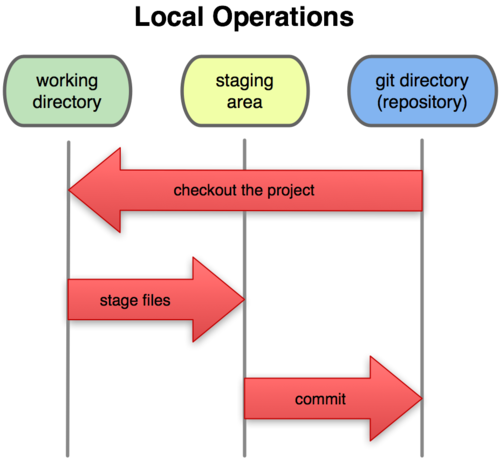
\includegraphics[width=7cm]{img/staging.png} \\
    Der Index ist sehr mächtig und Alleinstellungsmerkmal von git
  \end{center}
\end{frame}

\begin{frame}
  \frametitle{Der Index / Stage}
  \begin{center}
    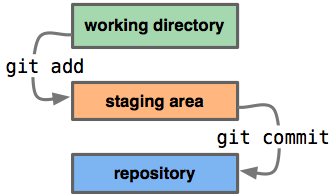
\includegraphics[width=5cm]{img/index1.png} \hspace{0.5cm} 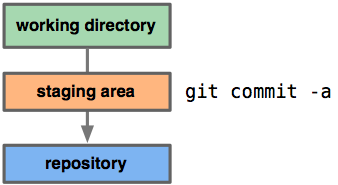
\includegraphics[width=5cm]{img/index2.png} \\
    \vspace{1cm}
    Typische Arbeitsweise mit git (links). \\ Workflow wie bei SVN (rechts) auch möglich.
  \end{center}
\end{frame}

\begin{frame}
  \frametitle{Dateizustände}
  \vspace{-0.3cm}
  \begin{center}
    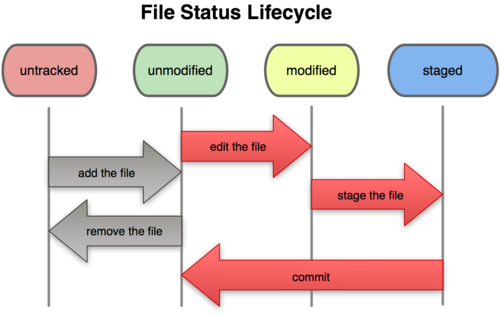
\includegraphics[width=10cm]{img/tracked.png} \\
    Anfangs evtl. verwirrend, {\tt git status} zeigt immer Hilfe an.
  \end{center}
\end{frame}

\begin{frame}
  \begin{center}
  \Huge Praxis \\
  \small Befehle, Dateien, Programme
  \end{center}
\end{frame}

\begin{frame}
  \frametitle{Wichtige git-Befehle - Arbeiten}
  \begin{itemize}
    \item {\tt git help <command>} \\ Hilfe zu git-commands, wichtigster Befehl ;)
    \item {\tt git init} \\ Ein git-Repo im aktuellen Verzeichnis beginnen
    \item {\tt git add} \\ Datei dem Index hinzufügen
    \item {\tt git status} \\ Status der Dateien im Arbeitsverzeichnis
    \item {\tt git diff} \\ Aktuelle Änderungen als diff anzeigen
    \item {\tt git commit} \\ Commit erstellen
  \end{itemize}
\end{frame}

\begin{frame}
  \frametitle{Wichtige git-Befehle - History}
  \begin{itemize}
    \item {\tt git log} \\ Log (History) anzeigen
    \item {\tt git branch} \\ Branches anzeigen (aktueller Branch hervorgehoben)
    \item {\tt git checkout <branch>} \\ Branch auschecken
    \item {\tt git show <object>} \\ Objekt (Branch, Commit, HEAD) anzeigen
    \item {\tt git blame -- <file>} \\ Anzeigen wer zuletzt welche Zeile geändert hat
  \end{itemize}
\end{frame}

\begin{frame}
  \frametitle{Wichtige git-Befehle - Kollaboration}
  \begin{itemize}
    \item {\tt git branch -a} \\ Alle Branches anzeigen
    \item {\tt git checkout -b <new\_branch> <old\_branch>} \\ Branch erzeugen und auschecken
    \item {\tt git pull} bzw. {\tt git fetch} \\ Aktualisierung des Repositories vom Server
    \item {\tt git push} \\ Aktualisierung des Repositories auf den Server
    \item {\tt git merge <branch>} \\ Einbinden eines anderen Branches
    \item {\tt git remote} \\ Anzeigen von eingetragenen Servern
  \end{itemize}
\end{frame}

\begin{frame}
  \frametitle{git revisions}
  \small Für Befehle wie {\tt git log, git diff, git checkout, git show} etc.
  \begin{itemize}
    \item {\tt dae86e1950b1277e545cee180551750029cfe735} oder {\tt dae86e} (falls eindeutig) \\ SHA1 des Commits
    \item {\tt master} oder {\tt origin/master} \\ Branch-Namen (References)
    \item {\tt master\~{}5} \\ Der fünfte Vorgänger des letzten Commits auf master
    \item {\tt master@\{yesterday\}} \\ Zustand von master gestern
  \end{itemize}
  Siehe auch {\tt git help rev-parse} für weitere Optionen
\end{frame}

\begin{frame}
  \frametitle{git revisions}
  \small Für Befehle wie {\tt git log, git diff} etc.
  \begin{itemize}
    \item {\tt master..testing} \\ Änderungen in testing aber nicht in master
    \item {\tt master..} \\ Änderungen im aktuellen Branch die nicht in master sind
    \item {\tt ..master} \\ Änderungen die in master aber nicht im aktuellen Branch sind
    \item {\tt master...testing} \\ Symmetrische Differenz
  \end{itemize}
  Siehe auch {\tt git help rev-parse} für weitere Optionen
\end{frame}


\begin{frame}
  \frametitle{Wichtige git-Dateien}
  \begin{itemize}
    \item {\tt \$HOME/.gitconfig} \\ git Benutzerkonfiguration 
    \item {\tt .gitignore} \\ Zum Ignorieren bestimmter Dateien bzw.\ Dateitypen, Verzeichnisweise und rekursiv
    \item {\tt .git} \\ git Repository, nur \emph{einmal}, im obersten Verzeichnis
    \item {\tt .git/config} \\ Konfiguration auf Repository-Ebene, z.B. Remotes
    \item {\tt .git/objects} \\ Objektdatenbank (Dateien, Commits, Tags)
    \item {\tt .git/refs} \\ Branches (References)
  \end{itemize}
\end{frame}

\begin{frame}
  \frametitle{Wichtige git-Dateien - Branches}
  Namespaces für refs (''references'') in {\tt .git}:
  \begin{itemize}
    \item {\tt .git/refs/heads} \\ Lokale Branches
    \item {\tt .git/refs/remotes} \\ Remote Branches
    \item {\tt .git/refs/tags} \\ Tags (Versionsnummern)
  \end{itemize}
  Gearbeitet wird \emph{immer} auf lokalen Branches, Remote Branches werden nur von {\tt git pull} bzw.\ {\tt git fetch} geändert. Commits ohne Branch gehen früher oder später verloren!
\end{frame}

\begin{frame}
  \frametitle{git Tutorial}
  Initiale Konfiguration: \\
  {\tt \small git config $--$global user.name ''Johannes Gilger''} \\ 
  {\tt \small git config $--$global user.email ''gilger@rz.de''} \\
  \vspace{0.5cm}
  Eventuell noch: \\
  {\tt \small git config $--$global color.ui ''auto''} \\ 
  {\tt \small git config $--$global color.status.changed ''yellow''} \\ 
\end{frame}

\begin{frame}
  \frametitle{Das erste Repository}
  \vspace{-0.3cm}
  \begin{center}
    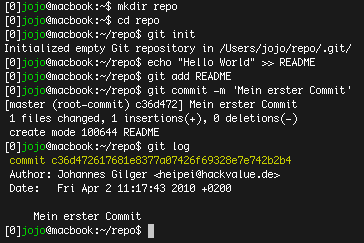
\includegraphics[width=8cm]{img/tutorial_1.png}
  \end{center}
\end{frame}

\begin{frame}
  \frametitle{Das erste Repository}
  \vspace{-0.3cm}
  \begin{center}
    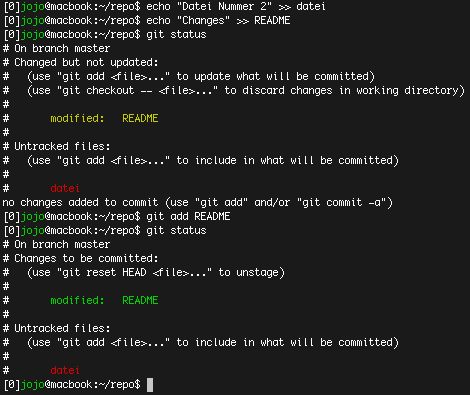
\includegraphics[width=9cm]{img/tutorial_2.png}
  \end{center}
\end{frame}

\begin{frame}
  \frametitle{Das erste Repository}
  \vspace{-0.3cm}
  \begin{center}
    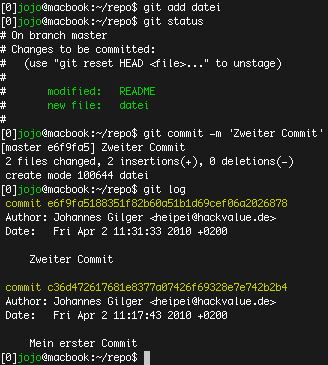
\includegraphics[width=6cm]{img/tutorial_3.png}
  \end{center}
\end{frame}

\begin{frame}
  \frametitle{git Installation \& Interfaces}
  \begin{itemize}
    \item {\bf Linux:} Installation mittels Distribution \\ Grafische Programme: {\tt gitk} und {\tt git gui}
    \item {\bf Mac OS X:} Installation mittels fink / MacPorts oder git-osx-installer \\ Grafische Programme: {\tt gitk} oder \href{http://gitx.frim.nl/}{GitX}
    \item {\bf Windows:} Installation per \href{http://code.google.com/p/msysgit/}{msysgit} \\ Grafische Programme: \href{http://code.google.com/p/tortoisegit/}{tortoisegit}
    \item {\bf Web:} GitWeb (privat), \href{http://github.com}{GitHub} (Hosted)
  \end{itemize}
  \begin{center}
  $\Rightarrow$ Wie immer ist die \href{http://git-scm.com}{git-Webseite} der beste Anlaufpunkt \\
  {\bf Aber:} Eigentlich kein GUI nötig um mit git zu arbeiten
  \end{center}

\end{frame}

\begin{frame}
  \frametitle{git GUIs - GitX}
  \vspace{-0.3cm}
  \begin{center}
    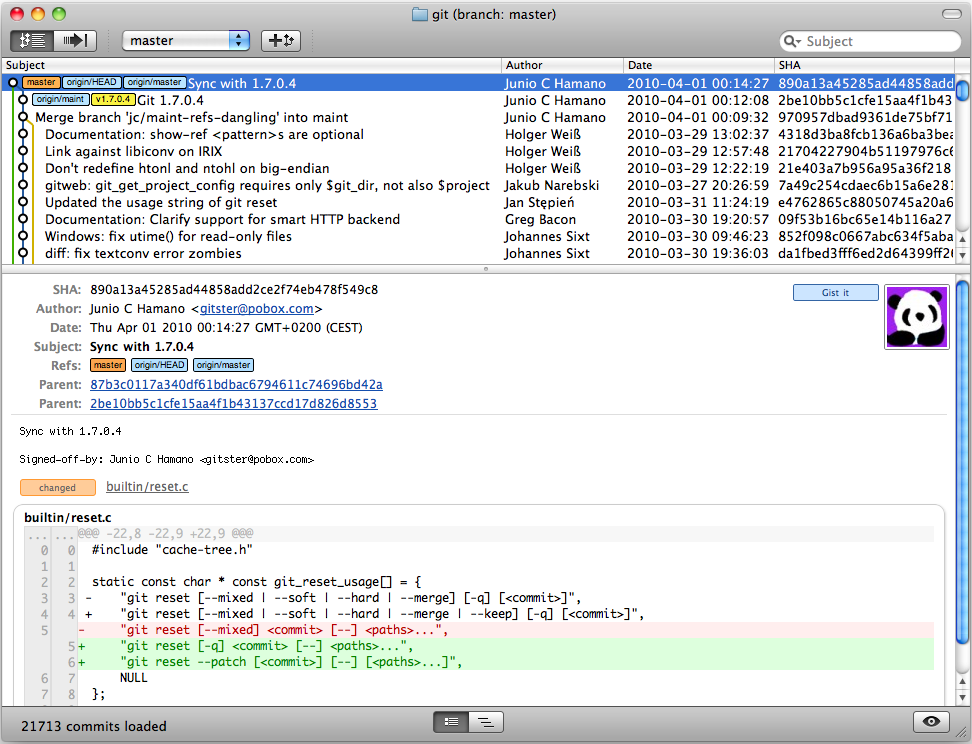
\includegraphics[width=9.5cm]{img/gitx.png}
  \end{center}
\end{frame}

\begin{frame}
  \frametitle{git GUIs - gitk}
  \vspace{-0.3cm}
  \begin{center}
    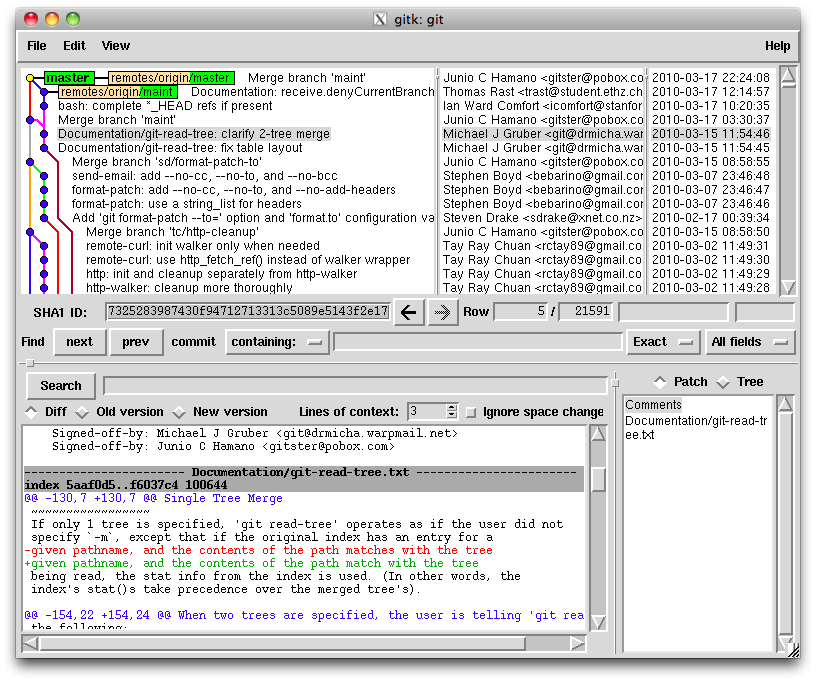
\includegraphics[width=9.0cm]{img/gitk.png}
  \end{center}
\end{frame}

\begin{frame}
  \frametitle{git GUIs - git gui}
  \vspace{-0.3cm}
  \begin{center}
    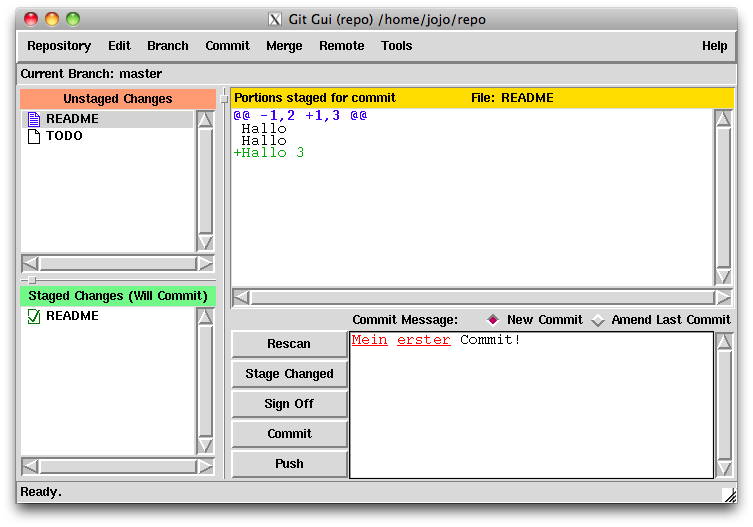
\includegraphics[width=9.5cm]{img/git_gui.png} \\
    Dateien können abschnittsweise committed werden
  \end{center}
\end{frame}

\begin{frame}
  \frametitle{git GUIs - tortoisegit}
  \vspace{-0.3cm}
  \begin{center}
    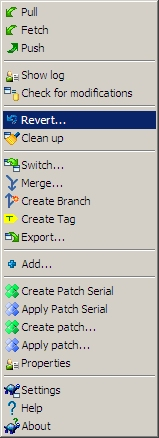
\includegraphics[width=2.5cm]{img/tortoisegit.png}
  \end{center}
\end{frame}

\begin{frame}
  \frametitle{git GUIs - tortoisegit}
  \vspace{-0.3cm}
  \begin{center}
    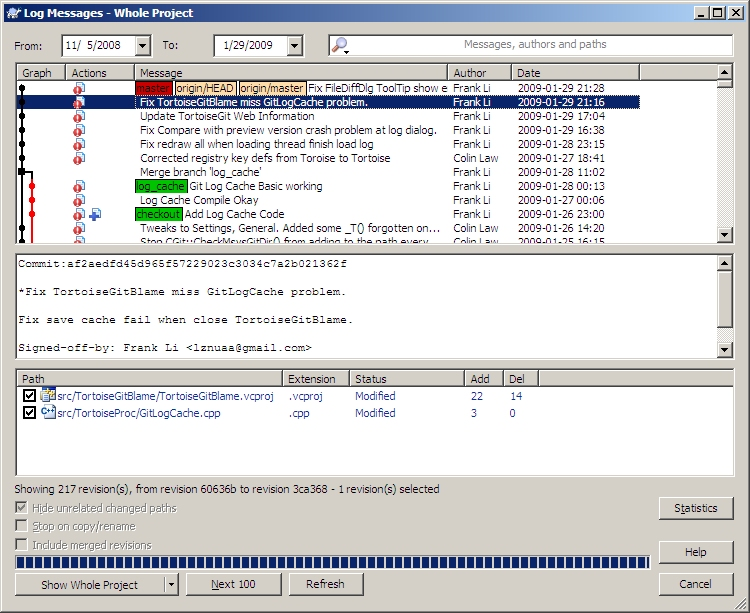
\includegraphics[width=9cm]{img/tortoisegit2.png}
  \end{center}
\end{frame}

\begin{frame}
  \frametitle{Wie wir im NOC git benutzen}
  \begin{itemize}
    \item {\bf Szenario 1:} Entwicklung (kleinerer) Webanwendungen \\ Meistens an Ort und Stelle (.git), sehr schnell und einfach
    \item {\bf Szenario 2:} Änderung an externer Software festhalten \\ (z.B.\ wenn Software von uns ''shibbolized'' wird)
    \item {\bf Szenario 3:} Größere Projekte mit mehreren Mitarbeitern. Ausgezeichnete Versionen (v0.5) direkt unterstützt
  \end{itemize}
\end{frame}

\begin{frame}
  \frametitle{Wie wir im NOC git benutzen}
  \vspace{-0.8cm}
  \begin{center}
    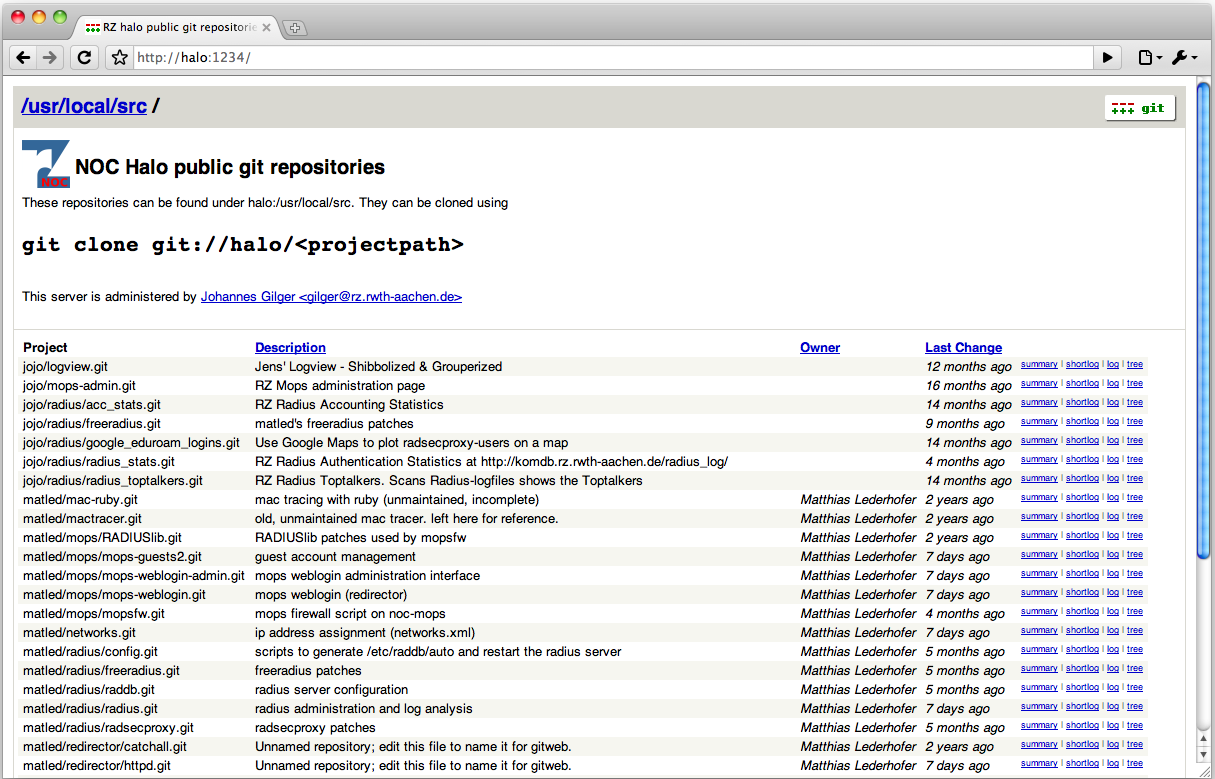
\includegraphics[width=11cm]{img/git_halo.png}
  \end{center}
\end{frame}

\begin{frame}
  \frametitle{Wie wir im NOC git benutzen}
  \vspace{-0.3cm}
  \begin{center}
    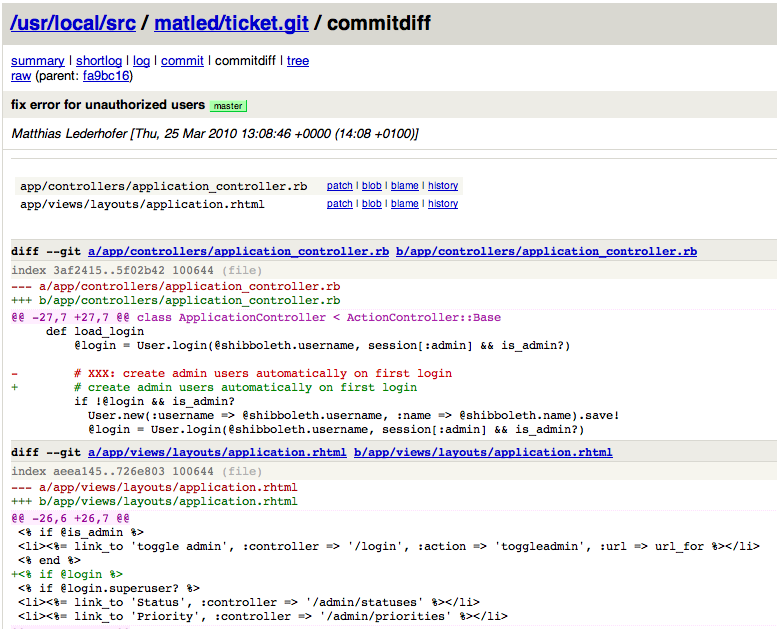
\includegraphics[width=9cm]{img/git_diff_halo.png}
  \end{center}
\end{frame}

\begin{frame}
  \frametitle{Benutzung von git lernen}
  \begin{enumerate}
    \item {\bf git installieren} \\ Linux: Package-Manager
    \item {\bf Kopie von bisherigem Code in neues Verzeichnis} \\ Dann ein {\tt git init} und weiterentwickeln
    \item {\bf Regelmäßig Doku / manpages lesen}
    \item {\bf Alle Befehle ausprobieren} \\ Insbesondere destruktive Aktionen und Recovery
    \item {\bf Im Zweifelsfall vorher das ganze Verzeichnis kopieren} \\ Als Backup wenn man sich noch nicht ganz sicher ist
    \item {\bf Dateien in {\tt .git} anschauen} \\ Was sind Objekte? Was sind Branches?
  \end{enumerate}
\end{frame}

\begin{frame}
  \frametitle{Literatur zu git}
  \begin{itemize}
    \item {\bf Pro Git} - \url{http://progit.org/book/} \\ Sehr ausführliches Online-Buch das alle Themen behandelt
    \item {\bf ''Getting Git''} - \url{http://www.gitcasts.com/git-talk} \\ Guter Vortrag (mit Folien) zur Benutzung und Datenstrukturen
    \item {\bf git ref} - \url{http://gitref.org/} \\ Die wichtigsten git-Befehle kurz erklärt
    \item {\bf git - SVN crash course} - \url{http://git-scm.com/course/svn.html} \\ Einführung in git mit Vergleichen zu svn
    \item {\bf Git - kurz \& gut} - O'Reilly, ISBN: 978-3-89721-914-4 \\ Gute und umfassende Einführung in Deutsch (\euro{9,90}) 
  \end{itemize}
\end{frame}

\begin{frame}
  \frametitle{The End}
  \begin{center}
  \Huge Fragerunde!
  \vspace{1.5cm}

  \small Folgefragen können gerne an gilger@rz.rwth-aachen.de und lederhofer@rz.rwth-aachen.de gerichtet werden. \\
  Oder einfach vorbei schauen ;)
  \end{center}
\end{frame}

\end{document}
